\documentclass[10pt,letterpaper]{article}

% ============================================================================
% Nature / bioRxiv Preprint Layout (XeLaTeX / Tectonic)
% Single unified Arial font matching all 6 Fignimble vector figures
% Strictly black typography: color appears exclusively in figures
% ============================================================================
\usepackage[letterpaper,left=0.82in,right=0.82in,top=0.74in,bottom=0.74in,headheight=19pt]{geometry}
\usepackage{fontspec}
\usepackage{amsmath,amssymb}
\usepackage{graphicx}
\usepackage{booktabs}
\usepackage{array}
\usepackage{tabularx}
\usepackage{xcolor}
\usepackage{caption}
\usepackage{titlesec}
\usepackage{fancyhdr}
\usepackage{lastpage}
\usepackage{enumitem}
\usepackage{microtype}
\usepackage[hidelinks]{hyperref}
\urlstyle{same}

% Single cohesive font family (Arial) across text and figures (Nature convention)
\setmainfont{Arial}[
  Scale=0.95,
  BoldFont={Arial Bold},
  ItalicFont={Arial Italic},
  BoldItalicFont={Arial Bold Italic}
]
\setsansfont{Arial}[Scale=0.95]
\setmonofont{Arial}[Scale=0.95]

% Clean journal reading rhythm and tight float-text co-placement
\linespread{1.11}
\setlength{\parindent}{0pt}
\setlength{\parskip}{4.4pt}
\setlength{\emergencystretch}{3em}
\renewcommand{\topfraction}{0.88}
\renewcommand{\bottomfraction}{0.80}
\renewcommand{\textfraction}{0.08}
\renewcommand{\floatpagefraction}{0.80}

% Monochrome black text throughout; subtle neutral gray only for hairlines
\definecolor{RuleGray}{HTML}{BDBDBD}
\color{black}

% Section and subsection headings: pure black, declarative, clean hierarchy
\titleformat{\section}
  {\fontsize{12.2}{15}\selectfont\bfseries\color{black}}
  {\thesection.}{0.5em}{}
  [\vspace{-3pt}\textcolor{RuleGray}{\rule{\textwidth}{0.5pt}}]
\titlespacing*{\section}{0pt}{14pt}{6pt}

\titleformat{\subsection}
  {\fontsize{10.8}{13.5}\selectfont\bfseries\color{black}}
  {\thesubsection}{0.55em}{}
  \titlespacing*{\subsection}{0pt}{10pt}{3.5pt}

% Nature-style captions (pure black Arial, bold label, ragged right)
\captionsetup{
  font={small,sf,color=black},
  labelfont={bf,color=black},
  labelsep=period,
  skip=6pt,
  justification=raggedright,
  singlelinecheck=false
}

% Running headers and footers (pure black)
\pagestyle{fancy}
\fancyhf{}
\renewcommand{\headrulewidth}{0.4pt}
\renewcommand{\headrule}{\hbox to\headwidth{\color{RuleGray}\leaders\hrule height \headrulewidth\hfill}}
\fancyhead[L]{\footnotesize\color{black}Koppikar (2026) \textbar\ Pan-prokaryotic +1 overprinted gene family in C5-cytosine methyltransferases}
\fancyhead[R]{\footnotesize\color{black}Preprint}
\fancyfoot[C]{\footnotesize\color{black}\thepage\ / \pageref{LastPage}}

\fancypagestyle{firstpage}{
  \fancyhf{}
  \renewcommand{\headrulewidth}{0pt}
  \fancyfoot[C]{\footnotesize\color{black}\thepage\ / \pageref{LastPage}}
}

% Semantic helpers (same Arial body font throughout; Nature superscript citations)
\newcommand{\spname}[1]{\textit{#1}}
\newcommand{\gene}[1]{\textit{#1}}
\newcommand{\refsup}[1]{\textsuperscript{#1}}

\begin{document}
\thispagestyle{firstpage}

% ============================================================================
% TITLE BLOCK
% ============================================================================
\noindent{\footnotesize\bfseries\color{black} PREPRINT \quad\textbar\quad COMPARATIVE GENOMICS AND STRUCTURAL EVOLUTION \quad\textbar\quad NOVEMBER 24, 2026}\\[5pt]
{\fontsize{15.0}{18.5}\selectfont\bfseries\color{black}\raggedright
A Pan-Prokaryotic and Viral +1 Overprinted Gene Family Inside Full-Length C5-Cytosine DNA Methyltransferases Explains the Origin of Split-Subunit Methyltransferases\par}
\vspace{5pt}

\noindent{\normalsize\color{black}
Pratik Koppikar\textsuperscript{1,*}\\[2pt]
{\small\color{black}
\textsuperscript{1}University of Cambridge, Cambridge, United Kingdom \;\textbar\; \textsuperscript{*}Correspondence: \href{mailto:psk34@cam.ac.uk}{psk34@cam.ac.uk} \;\textbar\; ORCID: \href{https://orcid.org/0000-0001-5089-5584}{0000-0001-5089-5584}\\
Code Availability: \url{https://github.com/koppikarp/c5mtase-plus1-overprint}\par
}}
\vspace{2pt}
\noindent{\color{RuleGray}\rule{\textwidth}{0.7pt}}
\vspace{4pt}

% ============================================================================
% ABSTRACT
% ============================================================================
\noindent{\fontsize{11.0}{13.8}\selectfont\bfseries\color{black} Abstract}
\vspace{2pt}

For three decades, the bacterial C5-cytosine DNA methyltransferases M.EcoHK31I and M.EaeI have been regarded as an isolated architectural curiosity in which a catalytically essential region, Motif IX, is relocated from the main enzyme onto a small overlapping polypeptide encoded in the +1 reading frame. Whether such dual-coding C5-methyltransferases represent a rare split-gene anomaly or point to a broader, unannotated protein family has remained unknown.

Here, through a frame-agnostic scan of 2,339 representative prokaryotic genomes (GTDB R232) and 5,063 complete bacteriophage genomes (INPHARED), we uncover a widespread +1 overprinted gene family embedded inside full-length, Motif-IX-intact C5-cytosine DNA methyltransferases across 13 prokaryotic phyla (spanning 11 bacterial and 2 DPANN archaeal phyla) and 17.0\% of all bacteriophage C5-methyltransferases (39/230 raw; 13.8\% dereplicated at $< 90\%$ catalytic-core identity, including 87.5\% raw and 83.3\% dereplicated of phage TPCQ enzymes). Remarkably, an unannotated member of this family resides inside the well-studied \gene{dmt} methyltransferase of model bacteriophage P1. Across divergent hosts, this +1 gene encodes a conserved CSLSDILE/KYFLS domain homologous to the N-terminal subunit-interaction region of M.EcoHK31I and M.EaeI $\beta$, yet terminates cleanly before Motif IX. Automated annotation pipelines systematically miss or erase the family: 29 of 33 audited UniProtKB matches among top MMseqs2 UniRef100 hits have been marked deleted, and the domain lacks any Pfam, InterPro, or experimental structural classification. Four orthogonal, non-pseudoreplicated evolutionary tests confirm purifying selection acting specifically on the +1 reading frame, including whole-gene composition-corrected conservation at non-stop-risk fourfold degenerate sites (gene-level paired Wilcoxon $P = 1.22 \times 10^{-4}$ across 13 FPCQ loci; independent replication $P = 1.56 \times 10^{-2}$ across 7 TPCQ/SPCQ loci) and non-circular, homology-selected stop-codon purging restricted to frame +1 (within-gene paired Wilcoxon max $P = 1.60 \times 10^{-3}$; $P = 1.53 \times 10^{-5}$ versus 1:1 GC3-matched homology-negative controls).

Outgroup-rooted maximum-likelihood phylogenies of both the host methyltransferase (97 unique taxa) and the harmonized CSLSDILE/KYFLS domain (67 taxa; 66 shared, Mantel $r = 0.56$ overall [$0.67$ excluding one long-branch outlier], $P = 0.0002$; non-overlapping C-terminal fusion Arch 3 subset $r = 0.75$, $P = 0.0004$) demonstrate that intact dual-coding is ancestral, whereas both textbook split-Motif-IX enzymes (M.EcoHK31I and M.EaeI) and single-chain C-terminal fusions found across four bacterial phyla represent single, younger derived transitions. AlphaFold 3 \textit{trans} co-folding across bacteria, archaea, and bacteriophage P1 predicts that the unlinked +1 polypeptide docks onto the exact Motif VIII, target-recognition-domain, and Motif IX collar occupied in \textit{cis} by C-terminal fusions (interface pTM 0.63--0.83; negative control M.HhaI 0.16), preserving a 3.69--4.04\,\AA\ contact between the conserved first arginine of Motif IX and the aromatic residue of KYFLS across all three architectures without occluding the catalytic cysteine ($\sim 22$--28\,\AA) or cofactor pocket ($\sim 19$\,\AA). This pre-existing \textit{trans} clamp provides a direct structural route for both Motif IX handoff into split subunits and de-overprinting into single-chain fusions, and yields immediately testable silent-frame-0, nonsense-+1 mutations in bacteriophage P1 \gene{dmt}.

\vspace{6pt}
\begin{figure}[!htbp]
  \centering
  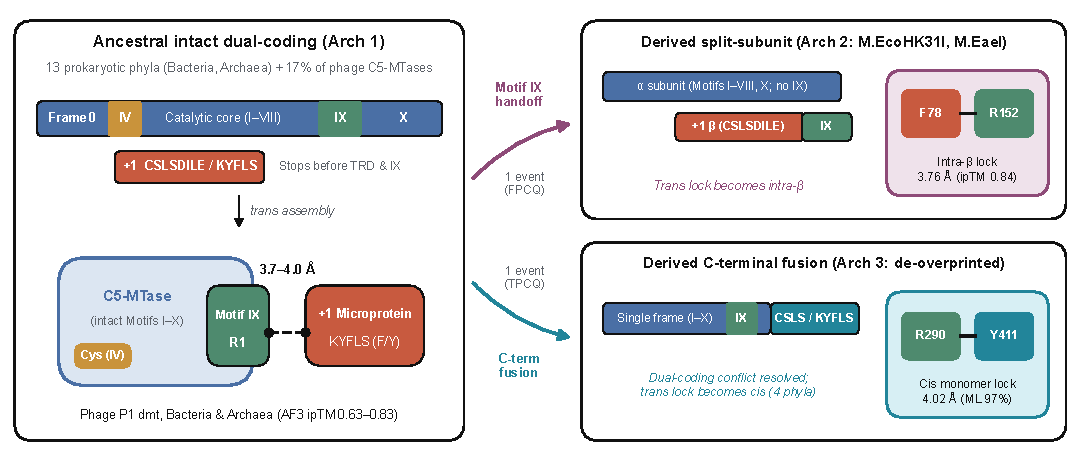
\includegraphics[width=\textwidth]{figures/rendered/graphical_abstract.pdf}
  \caption*{\textbf{Graphical Abstract.} Ancestral full-length, Motif-IX-intact C5-cytosine methyltransferases across bacteria, archaea, and bacteriophages carry an unannotated +1 overprinted CSLSDILE/KYFLS gene (Arch 1) predicted to dock in \textit{trans} at a conserved 3.7--4.0\,\AA\ Motif IX R1 to KYFLS F/Y interface. Two independent derived lineages converted this pre-existing \textit{trans} contact into either an intra-$\beta$ contact via Motif IX handoff (Arch 2: M.EcoHK31I, M.EaeI) or an intra-chain \textit{cis} contact via C-terminal fusion (Arch 3).}
\end{figure}

% ============================================================================
% 1. INTRODUCTION
% ============================================================================
\newpage
\section{Introduction}

Overlapping genes, in which a single segment of DNA encodes two distinct proteins in different reading frames, were first discovered in the compact single-stranded DNA bacteriophage $\phi$X174 nearly five decades ago\refsup{1} and are now recognized as major engines of genetic novelty across viruses\refsup{2--5}. Because every nucleotide in a dual-coding interval is constrained simultaneously by two amino-acid sequences, such ``overprinted'' genes evolve under unusually tight sequence constraints, often encoding small, rapidly adapting regulatory or accessory polypeptides\refsup{4,6}. Although ribosome profiling and evolutionary selection scans have begun to uncover translated overlapping genes in bacterial chromosomes as well\refsup{7--11}, prokaryotic and phage genome annotation pipelines (such as Prodigal and RefSeq/UniProt automated curation rules) explicitly penalize or suppress open reading frames (ORFs) nested inside longer conserved coding sequences\refsup{12,13}. As a result, deeply conserved overlapping genes embedded within well-known bacterial or viral enzymes are systematically filtered out of modern sequence databases.

Prokaryotic DNA (cytosine-5) methyltransferases (C5-MTases) are among the most thoroughly characterized enzyme families in molecular biology\refsup{14--17}. Found throughout restriction-modification systems and as ``orphan'' epigenetic regulators in bacterial chromosomes and bacteriophages\refsup{17,18}, C5-MTases catalyze the transfer of a methyl group from S-adenosyl-L-methionine (SAM) to the C5 carbon of cytosine by flipping the target base completely out of the DNA double helix\refsup{19,20}. Despite extensive sequence divergence, nearly all C5-MTases share ten conserved sequence motifs (Motifs I through X) arranged in a canonical order: Motifs I through VIII form the catalytic core (including the Motif IV PCQ active-site cysteine), a variable target recognition domain (TRD) determines DNA sequence specificity, and Motifs IX and X fold back onto the catalytic lobe to stabilize the TRD and organize the C-terminal collar\refsup{14,15,19,20}.

Since 1995, one striking exception to this single-polypeptide blueprint has dominated the biochemical literature: the \spname{Escherichia coli} HK31 methyltransferase M.EcoHK31I and its close homolog M.EaeI from \spname{Enterobacter} (\spname{Klebsiella}) \spname{aerogenes}\refsup{21--23}. Lee, Shaw, and colleagues demonstrated that M.EcoHK31I requires two polypeptides for activity: a 309-amino-acid $\alpha$ subunit carrying Motifs I--VIII and X, and a 176-amino-acid $\beta$ subunit encoded in the +1 overlapping reading frame of the $\alpha$ gene that supplies the missing Motif IX in \textit{trans}\refsup{21,22}. Subsequent biochemical dissection by Fung, Mak, Shaw, and colleagues showed that $\alpha$ alone forms non-productive aggregates with DNA, that $\beta$ binds $\alpha$ tightly ($K_d = 56.4$\,nM) to restore proper DNA engagement, and that deleting just 41 to 46 residues from the N-terminus of $\beta$ increases $K_d$ roughly 95-fold and abolishes enzymatic activity\refsup{24,25}. This natural split architecture later inspired engineered split C5-MTases for targeted epigenome editing\refsup{26}. Scattered subsequent genome annotations noted BLAST similarity to M.EcoHK31I $\alpha$ and $\beta$ in a conjugative transposon (\gene{Tn5252})\refsup{27} and in the temperate \spname{Streptococcus pneumoniae} bacteriophage MM1 (\gene{orf13}/\gene{orf14})\refsup{28}, yet those loci were interpreted simply as additional two-subunit M.EcoHK31I-like enzymes without auditing whether Motif IX remained intact in Frame 0. Consequently, for thirty years two fundamental questions have remained unanswered: how could an enzyme first split an essential conserved motif onto an out-of-frame polypeptide without passing through an inactive intermediate, and why did the $\beta$ subunit already possess a dedicated, high-affinity N-terminal subunit-interaction domain separate from Motif IX?

Here, we resolve both questions by showing that the N-terminal interaction domain of M.EcoHK31I and M.EaeI $\beta$ is actually one branch of a much larger, pan-prokaryotic and viral +1 overprinted gene family residing inside full-length, Motif-IX-intact C5-MTases (including phage MM1 \gene{orf13}/\gene{orf14} and the canonical \gene{dmt} methyltransferase of bacteriophage P1). Combining genomic surveys across GTDB R232 and INPHARED bacteriophages, unified composition-corrected synonymous-site selection statistics, outgroup-rooted maximum-likelihood phylogenetics, and AlphaFold 3 \textit{trans} co-folding, we establish the evolutionary sequence connecting intact dual-coding enzymes, split-subunit methyltransferases, and single-chain C-terminal fusions, and deliver an immediately testable experimental blueprint in bacteriophage P1.

% ============================================================================
% 2. RESULTS
% ============================================================================
\section{Results}

\subsection{A conserved +1 reading frame spans intact C5-methyltransferases across prokaryotes and phages}

To search systematically for unannotated dual-coding genes without relying on existing gene calls, we screened 2,339 high-quality representative bacterial and archaeal genomes from GTDB R232\refsup{29} (one representative per bacterial order or archaeal family, completeness $\ge 85\%$, contamination $\le 5\%$) for extended, stop-free alternate-frame ORFs nested inside conserved protein-coding genes. This screen uncovered a recurring, deeply conserved +1 reading frame spanning Motifs IV through VIII inside C5-cytosine DNA methyltransferases. Expanding the search across all 2,339 GTDB genomes by six-frame profile homology against both the newly identified +1 polypeptides and the N-terminal domain of M.EaeI $\beta$ (UniProt O52510) recovered 45 verified loci across 41 unique genomes, 41 distinct orders or families, and 13 prokaryotic phyla (11 bacterial phyla plus two DPANN archaeal phyla, \spname{Nanobdellota} and \spname{Aenigmatarchaeota}; Fig.~\ref{fig:fig1}a,b).

\begin{figure}[!htbp]
  \centering
  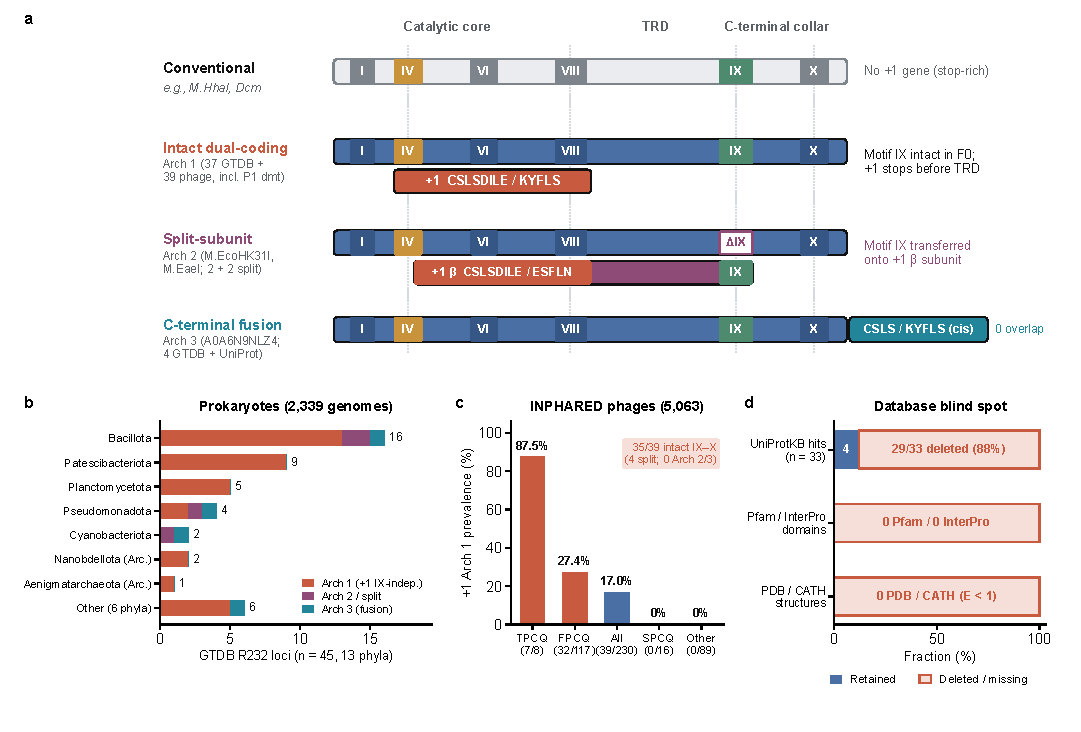
\includegraphics[width=\textwidth]{figures/rendered/fig1.pdf}
  \caption{\textbf{Three genomic architectures, taxonomic breadth, and database erasure of the CSLSDILE/KYFLS C5-methyltransferase family.} \textbf{a}, Domain and reading-frame alignment of conventional C5-MTases (top) against the three architectures carrying the CSLSDILE/KYFLS domain: intact dual-coding (Arch 1, Motif IX retained in Frame 0 while the +1 gene terminates before the TRD), split-subunit (Arch 2, M.EcoHK31I and M.EaeI, in which Motif IX is transferred onto the +1 $\beta$ subunit), and in-frame C-terminal fusion (Arch 3, A0A6N9NLZ4-type single-chain enzymes with zero reading-frame overlap). \textbf{b}, Distribution of all 45 verified GTDB R232 loci across all 13 prokaryotic phyla (11 bacterial and 2 DPANN archaeal: \spname{Nanobdellota} and \spname{Aenigmatarchaeota}), stacked by architecture. \textbf{c}, Prevalence of +1 Arch 1 loci across all 230 C5-MTases identified in 5,063 complete INPHARED bacteriophage genomes, stratified by exact Motif IV catalytic sequence (TPCQ 7/8, FPCQ 32/117, all 39/230, SPCQ 0/16, and all other variants 0/89); 35/39 phage hits reside inside continuous full-length Motif-IX/X-intact Frame-0 C5-MTases and 4/39 inside interrupted Frame-0 loci, with zero Arch 2 split-Motif-IX and zero Arch 3 fusions. \textbf{d}, Systematic erasure and annotation blind spots across audited UniProtKB matches among top MMseqs2 UniRef100 hits ($n = 33$), Pfam/InterPro, and experimental structure databases (PDB100/CATH50 via Foldseek).}
  \label{fig:fig1}
\end{figure}

Classifying every GTDB locus by reading frame and Motif IX position revealed three major genomic architectures and zero standalone copies outside C5-MTases (0/2,339 genomes; Fig.~\ref{fig:fig1}a,b). First, 37 of the 45 prokaryotic loci (82.2\%; 37/41 [90.2\%] of all overprinted loci) represent a widespread, Motif-IX-independent dual-coding architecture we term Arch 1: the embedded +1 gene spans roughly 135--170 codons across Motifs IV--VIII and terminates cleanly immediately after a conserved C-terminal core motif (CSLSDILE followed by [K/R][Y/F][F/Y]LS, hereafter CSLSDILE/KYFLS), never encoding Motif IX. Of these 37 Arch 1 loci, 35 sit inside continuous, full-length Frame-0 C5-MTases retaining intact Motifs I--VIII, a full TRD, and canonical Motifs IX and X in Frame 0 (spanning four catalytic Motif IV variants: FPCQ, TPCQ, SPCQ, and three \spname{Bacillota} SPCT enzymes), while 2 (\spname{Nanobdellota} GCA\_041653515.1 and \spname{Patescibacteriota} GCA\_963663305.1) sit inside frameshift- or contig-interrupted Motif-IX-intact FPCQ hosts. Across GTDB, Arch 1 occurs in \spname{Bacillota} (13 loci), \spname{Patescibacteriota} (9 loci), \spname{Planctomycetota} (5 loci), \spname{Pseudomonadota} (2 loci), \spname{Nanobdellota} (2 loci), \spname{Aenigmatarchaeota} (1 locus), and five additional bacterial phyla (\spname{Elusimicrobiota}, \spname{Desulfobacterota}, \spname{JACPUC01}, \spname{Myxococcota\_A}, and \spname{Chloroflexota}; 1 locus each). Second, 4 of the 45 GTDB loci (8.9\%) exhibit split-frame arrangements in which Motif IX is carried on the +1 polypeptide: 2 (4.4\%; one \spname{Thiotrichales} gammaproteobacterium and one \spname{Cyanobacteriota} genome) display the canonical M.EcoHK31I/M.EaeI Arch 2 architecture (Motif X retained in Frame 0, Motif IX fused to +1), while 2 paralogous \spname{SPCQ} loci in a single \spname{Bacillota} genome (GCA\_035934735.1) terminate Frame 0 after Motif VIII (223--224 aa) and run continuously in Frame +1 (475--477 aa) across CSLSDILE/KYFLS, the TRD, Motif IX, and Motif X (matching the split architecture of UniProt A0A136WGJ0). Third, 4 of the 45 GTDB loci (8.9\%), spanning four separate bacterial phyla (\spname{Bacteroidota}, \spname{Pseudomonadota}, \spname{Cyanobacteriota}, and \spname{Bacillota}), display a previously unrecognized de-overprinted architecture (Arch 3): a single, continuous Frame-0 polypeptide carrying intact Motifs I--X followed by a homologous CSLSDILE/KYFLS domain fused in-frame at the C-terminus (typified by \spname{Bacteroidota} UniProt entry A0A6N9NLZ4, 485 aa), with 3 to 5 stop codons in the +1 frame across Motifs VI--VIII and zero dual-coding overlap.

Genomic neighborhood audits ($\pm 5$ flanking ORFs around all GTDB loci) revealed frequent proximity to phage integrases, terminases, and mobile-element machinery rather than canonical restriction endonucleases alone, pointing toward bacteriophages as a major evolutionary reservoir. To test this directly, we scanned all 5,063 complete bacteriophage genomes in the INPHARED database\refsup{30}, identifying 230 phage-encoded C5-MTases. Strikingly, 39 of 230 phage C5-MTases (17.0\%) harbor the +1 CSLSDILE/KYFLS gene (Fig.~\ref{fig:fig1}c). Stratified by exact Motif IV class across all 230 phage enzymes, the +1 gene occurs in 7 of 8 phage TPCQ enzymes (87.5\%) and 32 of 117 phage FPCQ enzymes (27.4\%), while remaining absent from phage SPCQ enzymes (0/16; 0/18 including SPCT) and all other Motif IV variants combined (0/89, comprising 29 YPCQ, 15 IPCQ, 10 VPCS, 10 FPCT, and 25 minor variants). Crucially, this prevalence is not driven by clonal phage sampling: dereplicating all 230 phage C5-MTases by Frame-0 catalytic-core amino-acid identity yields 18/121 clusters (14.9\%; 0 mixed clusters) at $< 95\%$ identity, 15/109 clusters (13.8\%; TPCQ 5/6 [83.3\%], FPCQ 10/47 [21.3\%], SPCQ 0/10; 0 mixed clusters) at $< 90\%$ identity, and 11/92 clusters (12.0\%; TPCQ 5/6 [83.3\%]) at $< 80\%$ identity. All 39 phage hits encode the Motif-IX-independent +1 CSLSDILE/KYFLS gene (zero Arch 2 split-Motif-IX fusions and zero Arch 3 C-terminal fusions): 35 of 39 (89.7\%) reside inside continuous, full-length Motif-IX/X-intact Frame-0 ORFs (27 matching our strict Motif IX consensus and 8 full-length 328--507 aa enzymes retaining canonical Motif X and a divergent Motif IX in Frame 0), whereas 4 of 39 (10.3\%; AY129338, AY855346, KY065492, and EU719189) terminate Frame 0 early (247--276 aa) before a separate downstream or disrupted Motif IX--X segment. Notably, our INPHARED census recovers both the temperate \spname{S. pneumoniae} phage MM1 locus (AJ302074, \gene{orf13}/\gene{orf14}), previously annotated by BLAST similarity to M.EcoHK31I\refsup{28} yet here shown to be a continuous 385-aa full-length Arch 1 enzyme retaining canonical Motif IX (\texttt{RKLTPRECWRLQ}) and Motif X in Frame 0, and the well-characterized 754-aa \gene{dmt} methyltransferase of model \spname{Escherichia} bacteriophage P1 (GenBank AF234172; Swiss-Prot DAM\_BPP1)\refsup{31--33}, which contains a completely unannotated 163-codon stop-free +1 ORF (\texttt{CLLSQVLE...QRYFLS}) inside its N-terminal C5-MTase domain.

\subsection{Automated annotation pipelines and protein databases systematically erase the +1 gene family}

If this +1 gene occurs in roughly one-seventh of dereplicated phage C5-MTases and across 13 prokaryotic phyla, why has it escaped systematic recognition for three decades? Querying our conserved +1 polypeptide from \spname{Aneurinibacillales} (GCA\_002355375.1) against UniRef100 with MMseqs2\refsup{34} recovered 118 homologous entries. Auditing 33 representative non-UniParc UniProtKB accessions among high-coverage MMseqs2 hits (all $\ge 49\%$ query coverage plus top $E < 2.5 \times 10^{-10}$ UniProtKB matches; full accession table in repository data) revealed that 29 of 33 (87.9\%) have been marked obsolete and deleted from UniProtKB\refsup{13} during automated proteome cleanup of overlapping ORFs (Fig.~\ref{fig:fig1}d). Only four active entries survive among the 33 audited accessions: the annotated M.EaeI $\beta$ subunit (O52510), \spname{Streptococcus} phage P0093 entry A0A286QMS3, \spname{Paramagnetospirillum} entry M3AAZ1, and \spname{Streptococcus canis} entry A0A3P5XT20, all four carrying zero Pfam and zero InterPro annotations.

Furthermore, querying the CSLSDILE/KYFLS domain across InterPro and Pfam\refsup{35} returned zero domain families, and searching its AlphaFold DB monomer models (AF-O52510-F1 and AF-M3AAZ1-F1)\refsup{36} against the entire PDB100 and CATH50 structural databases using Foldseek\refsup{37} yielded zero experimental structural homologs ($E > 1.0$). Instead, the single top AlphaFold DB structural hit ($P = 1.000$) was the C-terminal extension of the Arch 3 in-frame fusion A0A6N9NLZ4 (485 aa), confirming that the overprinted +1 polypeptide and the C-terminal fusion domain share a previously uncharacterized fold systematically hidden by standard prokaryotic gene callers.

\subsection{Synonymous-site conservation and frame-specific stop purging confirm purifying selection in frame +1}

An extended stop-free ORF nested inside another gene can occasionally arise by chance in GC-rich genomes (where AT-rich stop codons TAA, TAG, and TGA are rare) or as a shadow of conserved amino-acid motifs in Frame 0. To distinguish genuine dual-coding purifying selection from compositional artifacts, RNA secondary structures, or pairwise pseudoreplication, we applied four orthogonal statistical tests strictly to homology-verified intact Arch 1 loci (Fig.~\ref{fig:fig2}).

\begin{figure}[!htbp]
  \centering
  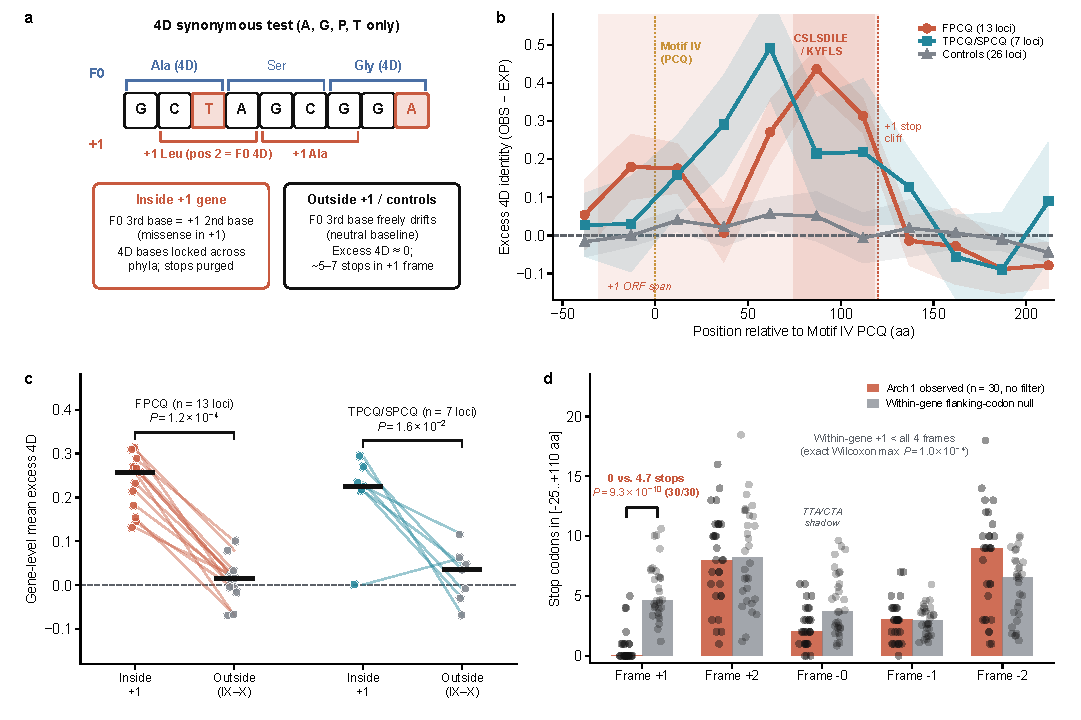
\includegraphics[width=\textwidth]{figures/rendered/fig2.pdf}
  \caption{\textbf{Orthogonal signatures of purifying selection acting specifically on the +1 reading frame of intact Arch 1 C5-methyltransferases.} \textbf{a}, Conceptual design of the non-stop-risk fourfold degenerate (4D) synonymous-site test restricted strictly to conserved alanine (A), glycine (G), proline (P), and threonine (T) codons in Frame 0: the third nucleotide is completely synonymous in Frame 0 and never creates a Frame-0 stop codon, yet constitutes the missense second codon position in Frame +1. \textbf{b}, Sliding-window (25-aa bins) whole-gene composition-corrected excess 4D identity (observed minus whole-gene A/G/P/T expected baseline across filtered 35--80\% Frame-0 AA-identity pairs; shading denotes $\pm 1$ genome-level cluster-bootstrap s.e.) relative to Motif IV PCQ (position 0) for Arch 1 FPCQ (terracotta, 13 independent loci, 51 pairs), independent Arch 1 TPCQ/SPCQ replication (petrol teal, 7 loci, 12 pairs; its peak offset at $+50..+74$ aa reflects a slightly more N-terminal Motif VI--VIII / +1 core spacing relative to Motif IV PCQ), and homology-negative +1-less controls (gray, 26 loci, 182 pairs). Excess conservation peaks over CSLSDILE/KYFLS and collapses at the +1 stop codon (+120 aa). \textbf{c}, Independent gene-level paired comparison of mean excess 4D identity inside the +1 span ($-30$ to $+120$ aa) versus outside in the conserved C-terminal Motifs IX--X (one observation per independent locus/genome; paired one-sided Wilcoxon signed-rank test: FPCQ $13/13$ inside $>$ outside, $P = 1.22 \times 10^{-4}$; TPCQ/SPCQ $6/7$, $P = 1.56 \times 10^{-2}$). \textbf{d}, Non-circular 5-frame stop-codon counts within $[-25..+110\text{ aa}]$ for strictly homology-selected low-GC Arch 1 loci ($\text{GC3} \le 0.38$, $n = 12$, zero stop-count filter) versus 1:1 nearest-GC3-matched homology-negative controls ($n = 12$, GC3 balance $P = 0.73$, zero stop-count filter). Frame +1 collapses to 0.0 stops (within-gene paired Wilcoxon versus all four other frames max $P = 1.60 \times 10^{-3}$; versus controls Mann--Whitney $U$ $P = 1.53 \times 10^{-5}$).}
  \label{fig:fig2}
\end{figure}

First, we evaluated synonymous-site conservation in Frame 0 strictly at conserved fourfold degenerate (4D) codons for alanine, glycine, proline, and threonine (A, G, P, and T; Fig.~\ref{fig:fig2}a). Restricting to A/G/P/T excludes valine (\texttt{GTN}, which can create +1 stops) while probing sites where the Frame-0 third base is completely neutral for the host enzyme yet serves as the missense second codon position in Frame +1\refsup{38,39}. To ensure complete consistency across sliding-window and paired analyses, we computed each pair's expected third-base identity ($\text{EXP}_{4D}$) once from whole-gene A/G/P/T third-base frequencies and applied the identical Frame-0 catalytic-core identity filter (35--80\% inside, 30--80\% outside) throughout, quantifying uncertainty via 2,000 genome-level cluster-bootstrap replicates. Across 13 independent low-to-moderate GC Arch 1 FPCQ loci ($\text{GC3} \le 0.45$, 51 cross-genome pairs), excess 4D identity climbs sharply across the +1 ORF, peaks at $+0.436$ (observed 4D identity 0.723 versus expected 0.287) directly over the CSLSDILE/KYFLS core ($+75$ to $+99$ aa relative to Motif IV), remains $+0.314$ across $+100$ to $+124$ aa, and drops abruptly to $-0.014$ immediately past the +1 stop codon ($+125$ to $+149$ aa; Fig.~\ref{fig:fig2}b). By contrast, 26 independent homology-negative control C5-MTases (182 pairs, selected with zero stop-count filter) remain flat near zero ($-0.045$ to $+0.056$) across the entire alignment.

Second, to eliminate pairwise pseudoreplication completely, we collapsed pairwise comparisons to one independent mean inside ($-30$ to $+120$ aa) and one independent mean outside (conserved C-terminal 75 aa containing Motifs IX--X) value per locus/genome. Every single Arch 1 FPCQ locus (13/13) exhibited higher excess 4D identity inside the +1 span than in its own C-terminal collar: gene-level median excess was $+0.258$ inside versus $+0.015$ outside (observed 0.537 versus 0.298; paired one-sided Wilcoxon signed-rank test, $P = 1.22 \times 10^{-4}$; Fig.~\ref{fig:fig2}c). Crucially, this localized signal replicated independently in the phylogenetically distant Arch 1 TPCQ/SPCQ subfamily (7 independent loci, 12 pairs; 6/7 inside $>$ outside, gene-level median excess $+0.225$ inside versus $+0.035$ outside; paired Wilcoxon $P = 1.56 \times 10^{-2}$; Fig.~\ref{fig:fig2}c). Direct between-group gene-level comparisons against the 26 homology-negative controls (median inside excess $+0.030$, outside $-0.037$) confirmed massive enrichment both in inside excess (Mann--Whitney $U$: FPCQ $P = 2.58 \times 10^{-7}$; TPCQ/SPCQ $P = 8.19 \times 10^{-4}$) and in the within-gene inside-minus-outside delta (FPCQ $P = 6.45 \times 10^{-7}$; TPCQ/SPCQ $P = 3.28 \times 10^{-3}$).

Third, to test frame-specific stop-codon purging without circular selection criteria, we selected all low-GC intact Arch 1 loci strictly by +1 sequence homology ($\text{GC3} \le 0.38$, $n = 12$, median GC3 0.260, zero stop-count filter) and counted stop codons across all five alternative reading frames ($+1$, $+2$, $-0$, $-1$, $-2$) within $[-25..+110\text{ aa}]$ (Fig.~\ref{fig:fig2}d). In our primary within-gene paired control (comparing all five frames inside the exact same DNA sequences), Frame +1 stop counts collapsed to a median of 0.0 (mean 0.4), significantly lower than every single other alternative frame: Frame +2 (median 11.0, paired Wilcoxon $P = 2.44 \times 10^{-4}$), Frame $-0$ (median 2.0, $P = 1.50 \times 10^{-3}$), Frame $-1$ (median 3.0, $P = 1.60 \times 10^{-3}$), and Frame $-2$ (median 9.5, $P = 2.44 \times 10^{-4}$). Comparing against 1:1 nearest-GC3-matched homology-negative C5-MTase controls ($n = 12$, median GC3 0.283, GC3 balance Mann--Whitney $U$ $P = 0.729$, also zero stop-count filter) confirmed an 8-stop selective collapse in Frame +1 (0.0 versus 8.0 stops; two-sided Mann--Whitney $U$ $P = 1.53 \times 10^{-5}$). Secondary reductions in Frames +2, $-0$, and $-1$ relative to controls (11.0 versus 15.0, 2.0 versus 6.5, and 3.0 versus 6.0) reflect dinucleotide and trinucleotide constraints imposed by locking the +1 coding sequence across Frame-0 codon boundaries, yet all four non-+1 frames remain heavily populated with premature stop codons, decisively ruling out frame-independent nucleic-acid structures.

Fourth, inspecting aligned columns within $[-30..+120\text{ aa}]$ where the Frame-0 amino acid diverged between cross-genome pairs showed that the overlapping +1 amino acid remained identical significantly more often in Arch 1 FPCQ loci than in homology-negative controls: collapsing to independent gene-level means yielded a median preservation rate of 18.4\% (mean 17.2\%, $n = 13$ loci) versus 10.7\% in controls (mean 11.0\%, $n = 26$ loci; one-sided Mann--Whitney $U$ $P = 2.40 \times 10^{-6}$, two-sided $P = 4.81 \times 10^{-6}$). Restricting further to maximum-cardinality disjoint non-overlapping pairs (zero genome reuse) confirmed the exact same enrichment (18.7\%, $n = 6$ pairs versus 10.4\%, $n = 10$ pairs; one-sided Mann--Whitney $U$ $P = 3.75 \times 10^{-3}$). Across all 10 strictly low-GC ($\text{GC3} \le 0.38$) homology-verified Arch 1 FPCQ loci spanning bacteria and DPANN archaea, six positions across L-S-D-I-L-E and the lysine of KYFLS (positions $+89$, $+91$, $+92$, $+93$, $+94$, and $+100$ relative to PCQ) were locked at 100\% third-base identity (10/10 lineages) despite extensive amino-acid turnover in Frame 0. Together, these four non-pseudoreplicated tests establish that the +1 ORF inside intact Arch 1 C5-MTases is a genuine, purifyingly selected protein-coding gene.

\subsection{Maximum-likelihood phylogenetics shows that intact dual-coding preceded split and fused architectures}

Finding the CSLSDILE/KYFLS domain in three genomic configurations (Arch 1 intact dual-coding, Arch 2 split-Motif-IX, and Arch 3 C-terminal fusion) raises a central evolutionary question: which architecture arose first? Three competing models are possible (Fig.~\ref{fig:fig3}a): split-subunit M.EcoHK31I-like enzymes (Arch 2) could be ancestral, single-chain fusions (Arch 3) could be ancestral and later overprinted, or intact dual-coding (Arch 1) could have originated first and subsequently given rise to both Arch 2 and Arch 3.

\begin{figure}[!htbp]
  \centering
  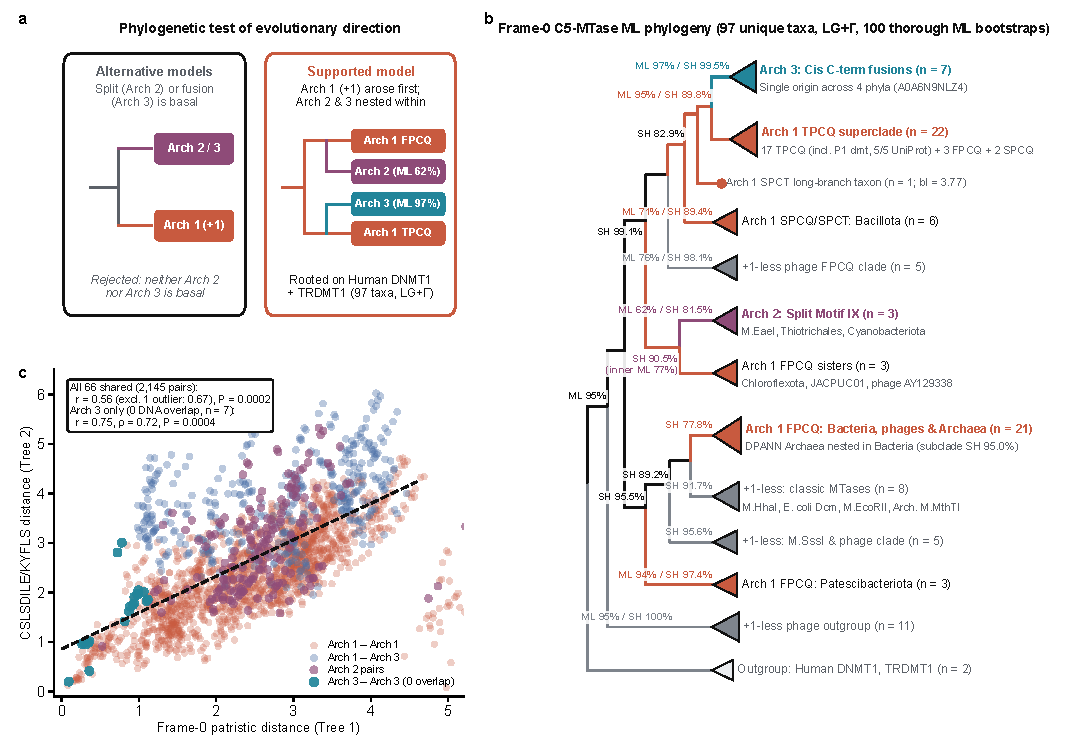
\includegraphics[width=\textwidth]{figures/rendered/fig3.pdf}
  \caption{\textbf{Outgroup-rooted maximum-likelihood phylogenetics establishes evolutionary direction from intact dual-coding (Arch 1) to derived split (Arch 2) and fused (Arch 3) lineages.} \textbf{a}, Competing evolutionary models tested by dual phylogenies. \textbf{b}, Frame-0 C5-MTase catalytic-core ML phylogeny (Tree 1; 97 unique non-redundant taxa, 185 MAFFT L-INS-i columns, VeryFastTree LG+$\Gamma$, 100 thorough ML bootstrap replicates plus SH-like local support) rooted strictly on human DNMT1 and TRDMT1/DNMT2. Minor sub-clades are collapsed to triangles summing strictly to 97 taxa; +1-less clades are labeled neutrally. Both Arch 2 (split Motif IX; ML 62\%, SH 81.5\%, nested with Arch 1 FPCQ sisters at inner ML 77\%, SH 91.9\% / 6-taxon SH 90.5\%) and Arch 3 (C-terminal fusions; ML 97\%, SH 99.5\%, nested inside a 100\%-CSLSDILE-carrying 29-taxon TPCQ superclade at ML 95\%, SH 89.8\%) are younger, monophyletic derived clades. Archaeal DPANN loci nest within bacterial Arch 1 FPCQ (subclade SH 95.0\%), indicating horizontal gene transfer. \textbf{c}, Pairwise patristic distance congruence between Tree 1 (Frame 0) and an independent harmonized ML tree of the CSLSDILE/KYFLS domain alone (Tree 2; 67 taxa, 77 columns) across all 66 shared taxa (2,145 pairs; Pearson $r = 0.56$ [$0.67$ excluding one long-branch outlier], Mantel $P = 0.0002$) and strictly within the zero-DNA-overlap Arch 3 subset ($n = 7$ taxa, 21 pairs; $r = 0.75$, $\rho = 0.72$, Mantel $P = 0.0004$).}
  \label{fig:fig3}
\end{figure}

To resolve this rigorously, we assembled two harmonized, deduplicated datasets combining GTDB R232 loci, INPHARED phages (removing duplicate Swiss-Prot Phage P1 DAM\_BPP1), UniProt Arch 2 and Arch 3 homologs, Swiss-Prot +1-less C5-MTase controls (including M.HhaI, \spname{E. coli} Dcm, M.EcoRII, M.SssI, and archaeal M.MthTI), and eukaryotic outgroups (human DNMT1 and TRDMT1/DNMT2). We aligned both datasets with MAFFT L-INS-i\refsup{40} and inferred maximum-likelihood trees under the LG+$\Gamma$ substitution model\refsup{41} in VeryFastTree\refsup{42,43}, applying identical thorough search settings (\texttt{-lg -gamma -spr 4 -mlacc 2 -slownni}) to both the main trees and all 100 non-parametric ML bootstrap replicates: Tree 1 on the Frame-0 catalytic core (97 unique taxa, 185 trimmed columns, strictly rooted on human DNMT1 and TRDMT1; Fig.~\ref{fig:fig3}b) and Tree 2 on the CSLSDILE/KYFLS domain itself (67 harmonized taxa sharing all 7 identical Arch 3 and all 3 Arch 2 representatives with Tree 1, 77 trimmed columns).

Before interpreting clade states, we audited five UniProt TPCQ entries that initially appeared to be +1-less controls in protein records (Swiss-Prot phage P1 DAM\_BPP1 plus four bacterial TrEMBL entries: W1J1U5, A0A068R437, A0A1Y2S7M7 from \spname{Xenorhabdus}, and A0A0J1C4Q1 from \spname{Neisseria arctica}; all five archived in repository data). Retrieving their underlying coding DNA from ENA and NCBI proved that 5 of 5 carry intact, unannotated 133--163 aa +1 CLLSQVLE/RYFLS ORFs. With all coding frames verified at the nucleotide level, Tree 1 and Tree 2 deliver four decisive evolutionary conclusions (Fig.~\ref{fig:fig3}b,c):

First, Arch 3 in-frame C-terminal fusions evolved once from an already-overprinted Arch 1 TPCQ ancestor. All 7 harmonized Arch 3 fusions spanning four bacterial phyla form a single tightly supported monophyletic clade in Tree 1 (ML bootstrap 97.0\%, SH 99.5\%) and independently in Tree 2 (ML 68.0\%, SH 94.6\%). Rather than sitting at the base of the tree, this Arch 3 clade nests deeply inside a strongly supported 29-taxon TPCQ superclade (ML 95.0\%, SH 89.8\%) in which 100\% of members (17 Arch 1 TPCQ enzymes including phage P1 \gene{dmt} and all DNA-verified UniProt TPCQ entries, 7 Arch 3 fusions, 3 phage FPCQ reverts, and 2 \spname{Planctomycetota} SPCQ enzymes) carry the CSLSDILE/KYFLS system. De-overprinting into a single-chain C-terminal fusion therefore resolved an ancestral dual-coding state rather than preceding it.

Second, textbook split-Motif-IX enzymes (Arch 2) also evolved once as a derived lineage, branching out of a separate Arch 1 FPCQ arm. All three Arch 2 taxa (M.EaeI, \spname{Thiotrichales}, and \spname{Cyanobacteriota}) cluster into one monophyletic clade (ML 62.0\%, SH 81.5\%) robustly nested with Arch 1 FPCQ sisters (inner 5-taxon clade with intact \spname{Chloroflexota} and \spname{JACPUC01} enzymes at ML 77.0\%, SH 91.9\%; 6-taxon clade including the interrupted Arch 1 bacteriophage AY129338 at SH 90.5\%). Crucially, sensitivity re-inference removing the single extreme long-branch taxon in Tree 1 (\texttt{A1\_SPCT\_Baci\_10645}, terminal branch length 3.77; 96 taxa, 100 thorough ML bootstraps) left every topology conclusion unchanged or stronger (Arch 3 monophyly ML 99.0\%, SH 99.6\%; TPCQ+Arch 3 superclade ML 95.0\%, SH 100.0\%; Arch 2 monophyly ML 61.0\%, SH 83.0\%), and midpoint rooting recovered the exact same nested placement of both Arch 2 and Arch 3.

Third, the Frame-0 methyltransferase and its +1 or C-terminal CSLSDILE/KYFLS domain co-evolved tightly across viral and cellular lineages (Fig.~\ref{fig:fig3}c). Across all 66 taxa shared between Tree 1 and Tree 2 (2,145 pairwise patristic distances), evolutionary distances correlate strongly (Pearson $r = 0.563$, Spearman $\rho = 0.606$, 5,000-permutation Mantel $P = 0.0002$; rising to $r = 0.674$, $\rho = 0.664$, $P = 0.0002$ when excluding the single long-branch outlier \texttt{A1\_SPCT\_Baci\_10645}). Because Frame 0 and Frame +1 share underlying DNA in Arch 1, we specifically tested non-overlapping pairs to rule out shared-DNA correlation: strictly within the 7 Arch 3 C-terminal fusion taxa (zero nucleotide overlap between the catalytic core and C-terminal domain; 21 pairs), patristic congruence is even stronger (Pearson $r = 0.749$, Spearman $\rho = 0.716$, Mantel $P = 0.0004$), and cross-architecture Arch 1-versus-Arch 3 pairs (392 cross-pairs, zero overlap in Arch 3) likewise correlate significantly ($r = 0.324$, $\rho = 0.389$, Mantel $P = 0.001$).

Fourth, the gene tree reflects phage- and mobile-element-driven horizontal gene transfer rather than vertical inheritance from the last universal common ancestor. Archaeal DPANN copies (\spname{Nanobdellota} and \spname{Aenigmatarchaeota}) nest cleanly inside a bacterial \spname{Patescibacteriota}/\spname{Elusimicrobiota} Arch 1 FPCQ subclade (SH 95.0\%). Meanwhile, conventional +1-less enzymes such as M.HhaI, \spname{E. coli} Dcm, M.EcoRII, archaeal M.MthTI (SH 91.7\%), and M.SssI (SH 95.6\%) form discrete +1-less clusters across the radiation. Because Fitch parsimony across the 95-taxon prokaryotic ingroup requires four binary transitions and leaves the deepest prokaryotic root state ambiguous (either +1-present or +1-absent), we label +1-less clades neutrally; our trees decisively establish a derived origin for Arch 2 and Arch 3 from Arch 1 and genuine co-evolution of the two domains without claiming that the earliest primordial C5-MTase was necessarily overprinted.

\subsection{Structure prediction models recover a conserved Motif IX arginine-to-aromatic clamp across all three architectures}

In the AlphaFold DB monomer model of the Arch 3 in-frame fusion A0A6N9NLZ4 (AF-A0A6N9NLZ4-F1, 485 aa)\refsup{36}, the C-terminal CSLSDILE/KYFLS core (residues 390--443) folds back onto the methyltransferase domain (residues 1--365), forming 83 inter-domain C$\alpha$--C$\alpha$ contacts ($< 8$\,\AA; 628 heavy-atom contacts $< 4.5$\,\AA; 186 C$\alpha$ and 1,151 heavy-atom contacts across the full C-terminal extension residues 366--485; minimum inter-domain PAE 1.0\,\AA) across Motif VIII, the TRD hinge, and Motif IX. This interface centers on a tight 4.02\,\AA\ C$\alpha$--C$\alpha$ contact between the conserved first arginine of Motif IX (R290) and the aromatic residue of KFYLS (Y411). This raised a crisp structural prediction: in full-length, Motif-IX-intact Arch 1 enzymes, does the separately translated +1 polypeptide physically dock in \textit{trans} onto that exact same Motif VIII/TRD/Motif IX collar?

\begin{figure}[!htbp]
  \centering
  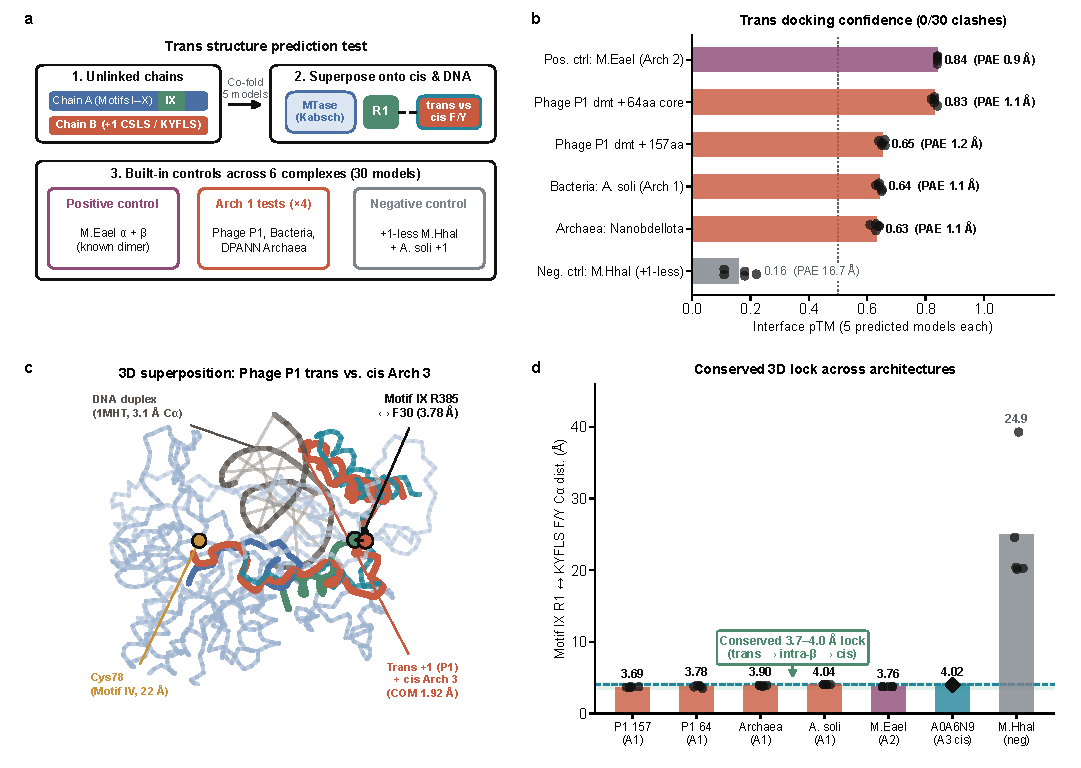
\includegraphics[width=\textwidth]{figures/rendered/fig4.pdf}
  \caption{\textbf{Structure prediction models reproduce the \textit{cis} Motif VIII/IX clamp and reveal a conserved 3.7--4.0\,\AA\ Motif IX R1 to KYFLS F/Y lock across all three architectures.} \textbf{a}, Conceptual design of the two-chain \textit{trans} co-folding test with built-in positive (M.EaeI $\alpha + \beta$) and negative (+1-less M.HhaI + \spname{A. soli} +1) controls across 6 complexes (30 independent models). \textbf{b}, Interface pTM (bars = 5-model mean, black dots = all 5 diffusion models) and mean minimum inter-chain PAE across all 6 complexes (0/30 atomic clashes). \textbf{c}, Atomic-coordinate 3D superposition using strictly rigid Rossmann-core anchors (excluding the mobile Motif IV base-flipping loop; 1MHT-to-A0A6N9NLZ4 core RMSD 0.84\,\AA) of the predicted Phage P1 \gene{dmt} + 64-aa +1 \textit{trans} complex (Frame-0 catalytic core in light slate, Motif VIII in slate, Motif IX in sage green, +1 microprotein in terracotta) onto the \textit{cis} Arch 3 domain of AF-A0A6N9NLZ4-F1 (petrol teal; 5-model center-of-mass distance $1.92 \pm 0.35$\,\AA) and the M.HhaI--DNA crystal structure (PDB 1MHT; DNA duplex in charcoal-sand flanking the TRD rim at $3.15 \pm 0.55$\,\AA\ C$\alpha$; catalytic Cys78 in ochre, 22\,\AA\ away). \textbf{d}, Conserved C$\alpha$--C$\alpha$ distance between Motif IX R1 and the homologous aromatic residue of KYFLS/RYFLS/ESFLN/KFYLS across all 5 models of every Arch 1 \textit{trans} complex, intra-$\beta$ Arch 2 (M.EaeI B:R152--F78), \textit{cis} Arch 3 (A0A6N9NLZ4 R290--Y411), and the negative control M.HhaI (24.9\,\AA).}
  \label{fig:fig4}
\end{figure}

We tested this hypothesis directly using AlphaFold Server (AlphaFold 3)\refsup{44} to co-fold six unlinked two-chain complexes (5 independent diffusion models per complex, 30 models total; Fig.~\ref{fig:fig4}a,b and Table~\ref{tab:af3}): four Motif-IX-intact Arch 1 pairs spanning all three evolutionary reservoirs (bacterial \spname{A. soli}, archaeal DPANN \spname{Nanobdellota}, and bacteriophage P1 \gene{dmt} paired with either its 157-aa or 64-aa SD+ATG +1 product), a positive control (experimentally verified heterodimer M.EaeI $\alpha + \beta$, Arch 2), and a negative control (+1-less M.HhaI, which possesses a canonical Motif IX and aligns within 0.69\,\AA\ rigid-core RMSD of A0A6N9NLZ4, paired with the \spname{A. soli} +1 polypeptide).

Across all 5 models per complex (zero clashes, 0/30), AlphaFold 3 cleanly separated true Arch 1 and Arch 2 complexes from the negative control (Fig.~\ref{fig:fig4}b and Table~\ref{tab:af3}). The positive control M.EaeI scored ipTM $0.840 \pm 0.000$ (minimum inter-chain PAE $0.92 \pm 0.01$\,\AA). All four full-length Motif-IX-intact Arch 1 pairs achieved high interface confidence (ipTM $0.630$--$0.830$; minimum inter-chain PAE $1.06$--$1.16$\,\AA; 5-model mean 837--1,454 heavy-atom contacts $< 4.5$\,\AA), with bacteriophage P1 \gene{dmt} + 64-aa +1 reaching ipTM $0.830 \pm 0.006$ (ranking score $0.910 \pm 0.006$), virtually matching M.EaeI. By contrast, +1-less M.HhaI rejected docking across all 5 models (ipTM $0.160 \pm 0.043$, minimum inter-chain PAE $16.68 \pm 2.67$\,\AA), confirming that AlphaFold 3 does not indiscriminately dock CSLSDILE/KYFLS onto arbitrary Motif-IX-bearing C5-MTases (while noting below that M.HhaI's +1-less clade also lacks paired-MSA co-evolutionary depth).

\begin{table}[!htbp]
\centering
\caption{\textbf{Predicted \textit{trans} co-folding benchmark across all 30 AlphaFold 3 diffusion models (5-model mean $\pm$ s.d. for every metric) compared with the \textit{cis} Arch 3 reference (AF-A0A6N9NLZ4-F1) and rigid-core superimposed M.HhaI--DNA (PDB 1MHT; core RMSD 0.84\,\AA).}}
\label{tab:af3}
\footnotesize
\renewcommand{\arraystretch}{1.18}
\resizebox{\textwidth}{!}{%
\begin{tabular}{@{}lccccccccc@{}}
\toprule
\textbf{Complex (Arch / Role)} & \textbf{Chains (aa)} & \textbf{ipTM} & \textbf{pTM} & \textbf{Rank} & \textbf{Min PAE (\AA)} & \textbf{R1--F/Y (\AA)} & \textbf{COM vs.\ \textit{cis} (\AA)} & \textbf{Dock RMSD (\AA)} & \textbf{DNA C$\alpha$ (\AA)} \\
\midrule
M.EaeI $\alpha + \beta$ (A2, pos.\ ctrl) & 309 + 176 & $0.840 \pm 0.000$ & $0.814 \pm 0.005$ & $0.938 \pm 0.004$ & $0.92 \pm 0.01$ & $3.76 \pm 0.01$ (intra-$\beta$) & $2.33 \pm 0.26$ & $4.03 \pm 0.18$ & $7.53 \pm 0.19$ \\
Phage P1 \gene{dmt} + 64aa (A1) & 473 + 64 & $0.830 \pm 0.006$ & $0.738 \pm 0.004$ & $0.910 \pm 0.006$ & $1.10 \pm 0.01$ & $3.78 \pm 0.15$ (\textit{trans}) & $1.92 \pm 0.35$ & $4.46 \pm 0.17$ & $3.15 \pm 0.55$ \\
Phage P1 \gene{dmt} + 157aa (A1) & 473 + 157 & $0.652 \pm 0.007$ & $0.734 \pm 0.005$ & $0.760 \pm 0.006$ & $1.16 \pm 0.02$ & $3.69 \pm 0.04$ (\textit{trans}) & $1.75 \pm 0.19$ & $4.35 \pm 0.10$ & $3.56 \pm 0.43$ \\
Bacteria \spname{A.\ soli} (A1) & 389 + 153 & $0.642 \pm 0.007$ & $0.686 \pm 0.005$ & $0.780 \pm 0.006$ & $1.13 \pm 0.01$ & $4.04 \pm 0.01$ (\textit{trans}) & $2.30 \pm 0.20$ & $4.43 \pm 0.13$ & $8.42 \pm 0.12$ \\
Archaea \spname{Nanobdellota} (A1) & 405 + 157 & $0.630 \pm 0.011$ & $0.630 \pm 0.009$ & $0.784 \pm 0.008$ & $1.06 \pm 0.02$ & $3.90 \pm 0.06$ (\textit{trans}) & $6.74 \pm 0.32$ & $13.22 \pm 0.69$ & $6.10 \pm 0.45$ \\
AF-A0A6N9NLZ4-F1 (A3, \textit{cis} ref) & 485 (1 ch) & \textemdash & \textemdash & \textemdash & 1.00 (inter-dom) & $4.02$ (\textit{cis}) & $0.00$ & $0.00$ & $4.12$ \\
M.HhaI + \spname{A.\ soli} +1 (neg.\ ctrl) & 327 + 153 & $0.160 \pm 0.043$ & $0.666 \pm 0.005$ & $0.418 \pm 0.036$ & $16.68 \pm 2.67$ & $24.93 \pm 7.37$ (none) & $17.87 \pm 8.51$ & $31.71 \pm 6.79$ & $5.72 \pm 8.27$ \\
\bottomrule
\end{tabular}}
\end{table}

Superimposing Chain A of all 30 models onto \textit{cis} AF-A0A6N9NLZ4-F1 using strictly rigid Rossmann-core anchors (Motifs IV $[-4..+1]$, VI, VIII, IX, and X, explicitly excluding the mobile Motif IV base-flipping loop M4$[+2..+8]$, which shifts $\sim 27$\,\AA\ upon DNA binding; Chain A core RMSD 0.49--1.51\,\AA, and 1MHT-to-A0A6N9NLZ4 core RMSD 0.84\,\AA\ across 46 C$\alpha$ atoms) revealed striking geometric convergence across all five diffusion models per complex (Fig.~\ref{fig:fig4}c,d and Table~\ref{tab:af3}). Without any covalent linker, the \textit{trans}-docked CSLSDILE/KYFLS core in phage P1 and bacterial \spname{A. soli} lands directly onto the \textit{cis} binding pocket across all 5 models (center-of-mass distance $1.75 \pm 0.19$\,\AA\ in P1 157-aa, $1.92 \pm 0.35$\,\AA\ in P1 64-aa, and $2.30 \pm 0.20$\,\AA\ in \spname{A. soli}; unaligned backbone docking RMSD $4.35$--$4.46$\,\AA, matching positive-control M.EaeI at COM $2.33 \pm 0.26$\,\AA\ and RMSD $4.03 \pm 0.18$\,\AA). In archaeal \spname{Nanobdellota}, the C-terminal flanking helices swing outward (COM $6.74 \pm 0.32$\,\AA, docking RMSD $13.22 \pm 0.69$\,\AA), yet the primary anchor contact remains locked in place. Most remarkably, in 20 of 20 Arch 1 \textit{trans} models, the exact homologous first arginine of Motif IX (R339 in \spname{A. soli}, R358 in \spname{Nanobdellota}, R385 in Phage P1 \gene{dmt}) packs against the exact homologous aromatic residue of KYFLS/RYFLS (F137, F126, and F123/F30) at $3.69$--$4.04$\,\AA\ C$\alpha$--C$\alpha$ (\spname{A. soli} $4.04 \pm 0.01$\,\AA\ versus \textit{cis} A0A6N9NLZ4 R290--Y411 at 4.02\,\AA; Fig.~\ref{fig:fig4}d). In Arch 2 M.EaeI, where Motif IX resides on the C-terminus of $\beta$, the exact same residue pair (B:R152--B:F78) is maintained at $3.76 \pm 0.01$\,\AA\ across all five models as an intra-subunit contact. Superimposing the ternary M.HhaI--DNA--SAH crystal structure (PDB 1MHT; 0.84\,\AA\ rigid-core RMSD)\refsup{20} places the CSLSDILE/KYFLS clamp far from the catalytic nucleophile (28.4\,\AA\ from Cys79 in \textit{cis} A0A6N9NLZ4, 22.3--23.5\,\AA\ from Cys78 in Phage P1 \gene{dmt}, and 27.6--28.0\,\AA\ in bacterial and archaeal Arch 1; equivalent to Cys81 in 1MHT) and far from the SAH cofactor (18.9--19.5\,\AA\ C$\alpha$), while positioning it directly along the DNA-facing TRD/Motif IX rim (3.15--8.42\,\AA\ C$\alpha$ and 1.20--4.62\,\AA\ heavy-atom distance to superimposed apo-docked 1MHT DNA, compared with 4.12\,\AA\ C$\alpha$ / 3.50\,\AA\ heavy in \textit{cis} A0A6N9NLZ4; Fig.~\ref{fig:fig4}c).

\subsection{Bacteriophage P1 dmt encodes a compact +1 microprotein core ready for genetic validation in Escherichia coli}

The discovery of an Arch 1 locus inside \gene{dmt} of bacteriophage P1 (GenBank AF234172: 66,412--68,676, + strand, 754 aa; Fig.~\ref{fig:fig5}a) places this gene family inside one of the most genetically tractable workhorses of \spname{E. coli} molecular biology\refsup{31--33}. In phage P1, Dmt is a two-domain fusion comprising an N-terminal C5-MTase domain (residues 1--473, with intact Motifs I--X including active-site Cys78 and Motif IX R385) linked to a C-terminal N6-adenine Dam methyltransferase domain (residues 485--754) required for \gene{pac}-site methylation and phage DNA packaging\refsup{31--33}. Nested inside the C5-MTase domain lies an unannotated 163-codon stop-free +1 ORF (AF234172: 66,710--67,201; \gene{dmt} nucleotides 299--790) carrying two internal in-frame ATG codons preceded by canonical GGAG Shine--Dalgarno ribosome-binding motifs: one at nucleotide 66,728 (7-nt spacer, predicting a 157-aa polypeptide) and a second at nucleotide 67,007 (8-nt spacer, predicting a compact 64-aa microprotein beginning immediately upstream of CLLSQVLE...RYFLS).

\begin{figure}[!htbp]
  \centering
  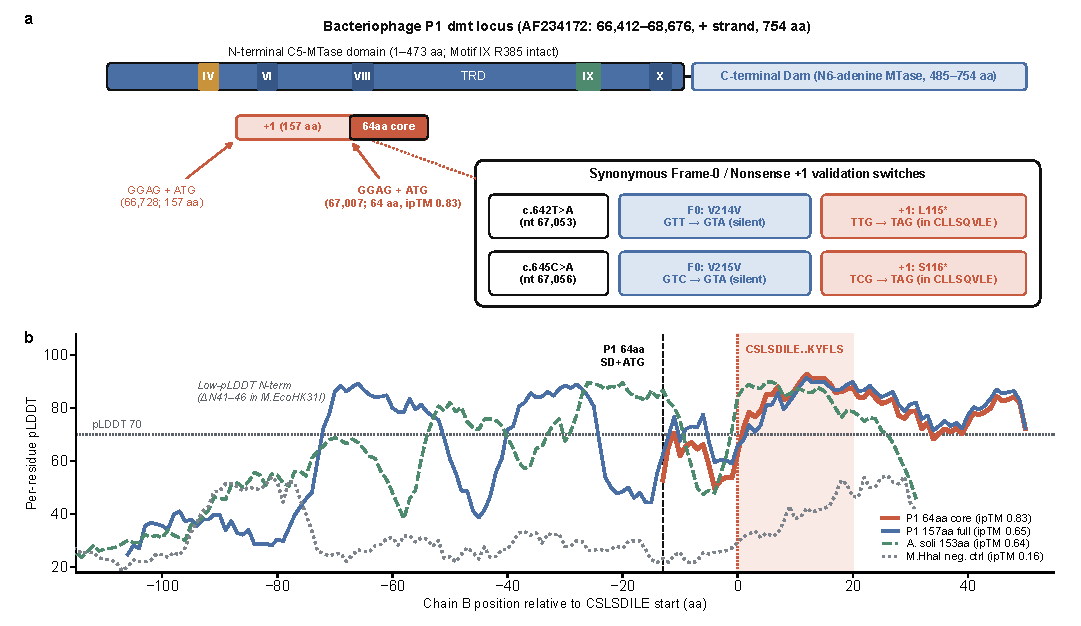
\includegraphics[width=\textwidth]{figures/rendered/fig5.pdf}
  \caption{\textbf{Bacteriophage P1 \gene{dmt} harbors a compact +1 microprotein core and provides single-nucleotide synonymous validation switches.} \textbf{a}, To-scale map of phage P1 \gene{dmt} (AF234172: 66,412--68,676, 754 aa), highlighting the N-terminal C5-MTase domain (slate blue, Motifs IV--X intact), C-terminal Dam adenine methyltransferase domain (light slate), and embedded +1 ORF with its two internal GGAG Shine--Dalgarno + ATG start sites (157 aa and 64 aa core). Inset shows the two primary codon-neutral single-nucleotide mutations (\gene{dmt} c.642T$>$A and c.645C$>$A) that are completely synonymous in Frame 0 (V214V, V215V) while introducing premature amber stop codons inside CLLSQVLE in Frame +1 (L115*, S116*). \textbf{b}, Per-residue pLDDT profiles across Chain B aligned at the start of CSLSDILE (position 0), showing a low-pLDDT N-terminal region matching the biochemically dispensable $\Delta$N41--46 boundary of M.EcoHK31I $\beta$\refsup{24} and a sharp pLDDT rise right at the 64-aa SD+ATG start (vertical dashed line) that elevates ipTM from 0.65 to 0.83.}
  \label{fig:fig5}
\end{figure}

Inspecting per-residue pLDDT profiles across all full-length Arch 1 +1 chains explains why trimming the phage P1 +1 product from 157 aa to the 64-aa SD+ATG core elevated ipTM from $0.652$ to $0.830$ (Fig.~\ref{fig:fig5}b). Across phage P1, \spname{A. soli}, and \spname{Nanobdellota}, the N-terminal half of the stop-to-stop +1 span exhibits low structural confidence (mean pLDDT 43.6--58.9), whereas pLDDT rises sharply over the C-terminal WMNW--CSLSDILE--KYFLS core (78.5--84.5). This boundary mirrors both the sharp downstream peak of our 4D synonymous conservation scan ($+75$ to $+120$ aa; Fig.~\ref{fig:fig2}b) and the published N-terminal deletion mapping of M.EcoHK31I $\beta$ by Fung et al.\refsup{24}, where deleting residues 1--41 was tolerated (16-fold activity drop) whereas extending deletion to residue 46 (cutting directly into the conserved Motif VIII-contacting helix upstream of CTLSQVLE) increased $K_d$ 95-fold and inactivated the enzyme. Together, these observations raise the testable hypothesis that the active translated product in many Arch 1 loci may be a compact 64--85 aa microprotein initiated from an internal Shine--Dalgarno site rather than the entire stop-to-stop span.

To enable genetic perturbation without altering a single amino acid of Frame-0 P1 Dmt, we verified four single-nucleotide substitutions within CLLSQVLE...RYFLS directly against the AF234172 coding sequence that are strictly synonymous in Frame 0 while introducing premature amber (\texttt{TAG}) stop codons in Frame +1 (Table~\ref{tab:p1mut} and Fig.~\ref{fig:fig5}a). We prioritize c.642T$>$A (V214V, \texttt{GTT} $\rightarrow$ \texttt{GTA}; moderate \spname{E. coli} usage 10.9/1,000) and c.645C$>$A (V215V, \texttt{GTC} $\rightarrow$ \texttt{GTA}; 10.9/1,000) as primary alleles because both terminate the +1 gene directly inside \texttt{CLLSQVLE} without introducing rare \spname{E. coli} codons, whereas the two downstream alleles (c.666C$>$A introducing rare Leu codon \texttt{CTA}, 3.9/1,000; c.714T$>$A introducing rare Ile codon \texttt{ATA}, 4.4/1,000) serve as secondary alleles. Because all four nonsense mutations generate \texttt{TAG} stops, genetic tests should be conducted in a non-amber-suppressor (\gene{sup}$^0$) \spname{E. coli} host (such as MG1655, W3110, or BL21), avoiding \gene{supE44}/\gene{glnV} suppressor strains (such as C600, DH5$\alpha$, or JM109).

\begin{table}[!htbp]
\centering
\caption{\textbf{Verified single-nucleotide validation mutations in bacteriophage P1 \gene{dmt} (GenBank AF234172) that knock out the +1 reading frame via amber (\texttt{TAG}) stops without altering Frame-0 Dmt. Perform assays in a non-amber-suppressor (\gene{sup}$^0$) \spname{E. coli} host (e.g., MG1655, W3110, BL21).}}
\label{tab:p1mut}
\footnotesize
\renewcommand{\arraystretch}{1.18}
\resizebox{\textwidth}{!}{%
\begin{tabular}{@{}lllllll@{}}
\toprule
\textbf{\gene{dmt} nt} & \textbf{AF234172} & \textbf{Sub.} & \textbf{Frame-0 Dmt (codon; \spname{E. coli} usage)} & \textbf{Frame +1 (163-aa / 64-aa)} & \textbf{Location in +1} & \textbf{Priority} \\
\midrule
c.642 & 67,053 & T $>$ A & V214V (\texttt{GTT} $\rightarrow$ \texttt{GTA}; moderate 10.9/1k) & L115* / L16* (\texttt{TTG} $\rightarrow$ \texttt{TAG}) & Inside \texttt{CLLSQVLE} core & Primary \\
c.645 & 67,056 & C $>$ A & V215V (\texttt{GTC} $\rightarrow$ \texttt{GTA}; moderate 10.9/1k) & S116* / S17* (\texttt{TCG} $\rightarrow$ \texttt{TAG}) & Inside \texttt{CLLSQVLE} core & Primary \\
c.666 & 67,077 & C $>$ A & L222L (\texttt{CTC} $\rightarrow$ \texttt{CTA}; rare 3.9/1k) & S123* / S24* (\texttt{TCG} $\rightarrow$ \texttt{TAG}) & Linker before \texttt{RYFLS} & Secondary \\
c.714 & 67,125 & T $>$ A & I238I (\texttt{ATT} $\rightarrow$ \texttt{ATA}; rare 4.4/1k) & L139* / L40* (\texttt{TTG} $\rightarrow$ \texttt{TAG}) & C-terminal packing helix & Secondary \\
\bottomrule
\end{tabular}}
\end{table}

% ============================================================================
% 3. DISCUSSION
% ============================================================================
\clearpage
\section{Discussion}

\subsection{A unified structural mechanism for the evolution of split-subunit and fused C5-methyltransferases}

For thirty years, the split-subunit methyltransferases M.EcoHK31I and M.EaeI posed an evolutionary puzzle: how could a single-chain C5-MTase lose its essential Motif IX from Frame 0 and transfer it onto a +1 overlapping $\beta$ subunit without traversing a dead, non-functional intermediate? Our phylogenetic and structural findings resolve this paradox through a simple, three-step evolutionary sequence (Graphical Abstract). First, an ancestral full-length C5-MTase acquired a +1 overprinted CSLSDILE/KYFLS gene (Arch 1) whose polypeptide product docked in \textit{trans} onto the Motif VIII, TRD, and Motif IX collar, establishing a conserved 3.7--4.0\,\AA\ contact directly against the first arginine of Motif IX. Second, once this \textit{trans} clamp already bridged Motif VIII and Motif IX, two opposite evolutionary resolutions became structurally accessible without needing to invent a new protein--protein interface: on one FPCQ branch (Arch 2, M.EcoHK31I/M.EaeI), transferring Motif IX from the C-terminus of $\alpha$ onto the C-terminus of the +1 $\beta$ subunit simply converted the pre-existing \textit{trans} R1--F/Y lock into an intra-$\beta$ contact (3.76\,\AA); on an independent TPCQ branch (Arch 3, A0A6N9NLZ4 and relatives across four phyla), relocating the CSLSDILE/KYFLS coding segment to the C-terminus of Frame 0 eliminated dual-coding mutational conflict while converting the exact same \textit{trans} contact into an intra-chain \textit{cis} lock (4.02\,\AA). The discovery of two \spname{Bacillota} paralogs (GCA\_035934735.1) in which Frame 0 terminates after Motif VIII and Frame +1 extends continuously through CSLSDILE/KYFLS, the TRD, Motif IX, and Motif X further illustrates how readily this pre-existing +1 architecture accommodates alternative split-frame transitions.

This model also illuminates prior experimental biochemistry on M.EcoHK31I. Fung et al.\refsup{24} demonstrated in 2006 that purified M.EcoHK31I $\alpha$ forms non-productive aggregates with DNA in the absence of $\beta$, and that N-terminal truncation of $\beta$ at residue 46 causes a 95-fold loss of binding affinity ($K_d$ rising from 56.4\,nM) and complete loss of catalysis. Mapping those boundaries onto our AlphaFold 3 models shows that residues 42--80 of $\beta$ constitute precisely the conserved Motif VIII- and Motif IX-clamping WMNW--CSLSDILE--KYFLS core shared across all Arch 1 and Arch 3 homologs. Thus, the tight subunit-interaction module characterized biochemically in M.EcoHK31I $\beta$ did not evolve specifically to support a split Motif IX; rather, it predated the split and physically enabled it.

\subsection{Systematic blind spots in prokaryotic and viral proteome databases}

Our audit highlights an ongoing failure mode in automated genome annotation. Because standard prokaryotic gene callers (Prodigal, PGAP) and UniProt redundancy filters aggressively remove ORFs overlapping conserved enzymes\refsup{12,13}, nearly 90\% (29/33) of audited UniProtKB matches among top MMseqs2 CSLSDILE/KYFLS hits have already been purged from UniProtKB, and zero Pfam/InterPro entries exist despite the domain spanning 13 prokaryotic phyla and 17.0\% of phage C5-MTases (13.8\% dereplicated at $< 90\%$ identity). Strikingly, even four UniProt bacterial TPCQ methyltransferases we initially selected as +1-less controls, alongside the 2004 reference annotation of bacteriophage P1 \gene{dmt}\refsup{31}, proved upon nucleotide inspection to carry intact +1 ORFs, while prior annotations of phage MM1 \gene{orf13}/\gene{orf14}\refsup{28} missed that Motif IX remains intact in Frame 0. As large-scale metagenomic and phage cataloging accelerates, integrating frame-agnostic synonymous-site conservation metrics (such as non-stop-risk 4D tests, OLGenie, or Synplot2)\refsup{9,38,39} directly into annotation pipelines will be essential to halt the systematic deletion of conserved prokaryotic and viral microproteins\refsup{10,11}.

\subsection{Scope, structural modeling limitations, and open mechanistic hypotheses}

We emphasize clear boundaries between what our computational evidence establishes and what requires experimental proof. First, four independent, non-pseudoreplicated evolutionary signatures (whole-gene composition-corrected A/G/P/T 4D conservation, independent subfamily replication, non-circular homology-selected stop purging, and +1 amino-acid preservation across host-mutated sites) plus ML phylogenetic nesting and zero-DNA-overlap Arch 3 patristic congruence ($r = 0.75$) prove beyond reasonable doubt that the +1 CSLSDILE/KYFLS gene in full-length Arch 1 C5-MTases is under strong protein-level purifying selection and predates both Arch 2 and Arch 3.

Second, our \textit{trans} structure predictions (ipTM 0.63--0.83 across 20/20 Arch 1 models versus 0.16 for M.HhaI) provide strong structural and co-evolutionary support for a conserved Motif VIII/TRD/Motif IX clamp, but carry two important methodological caveats: AlphaFold 3 constructs paired multiple sequence alignments that can draw inter-residue co-evolutionary couplings from both \textit{cis} Arch 3 fusions and \textit{trans} Arch 2 operons, and conversely the negative control M.HhaI belongs to a +1-less clade with zero paired-MSA depth for a cognate +1 partner. Consequently, structural modeling demonstrates biophysical compatibility and conserved interface geometry, not physical proof of \textit{in vivo} translation or heterodimer formation in Arch 1 loci.

Third, the physiological function of the CSLSDILE/KYFLS clamp in full-length, Motif-IX-intact enzymes (both Arch 1 and Arch 3) remains an open question. Unlike M.EcoHK31I, where $\beta$ is catalytically indispensable because it supplies Motif IX, Arch 1 and Arch 3 enzymes already encode an intact Motif IX in Frame 0. With our rigid-core 1MHT superposition (0.84\,\AA\ RMSD) showing that the clamp lies remote from the active-site cysteine ($\sim 22$--28\,\AA) and SAH ($\sim 19$\,\AA) yet sits immediately adjacent to the DNA-facing TRD/Motif IX rim (3.2--8.4\,\AA\ C$\alpha$ to superimposed apo-docked 1MHT DNA), and given the DNA-aggregation phenotype observed when M.EcoHK31I $\alpha$ lacks $\beta$\refsup{24}, three non-exclusive mechanistic hypotheses merit testing: (i) a folding or anti-aggregation chaperone that stabilizes the flexible TRD--Motif IX collar during DNA engagement; (ii) a DNA-rim modulator or allosteric regulator tuning methylation kinetics, target engagement, or timing (particularly intriguing in phage P1 \gene{dmt}, where DNA methylation gates \gene{pac} cleavage and lytic versus lysogenic development\refsup{31--33}); or (iii) a structural shield protecting the exposed C-terminal collar against host proteases or anti-methyltransferase defense systems during phage--host conflict. Because bacteriophage P1 is readily tractable in \gene{sup}$^0$ \spname{E. coli}, C-terminal epitope tagging of the +1 ORF, co-immunoprecipitation of the predicted R385--F30 interface, and phenotyping of our prioritized synonymous Frame-0 / nonsense +1 knockouts (Table~\ref{tab:p1mut}) with \textit{trans} complementation can resolve expression, physical binding, and biological function directly at the bench.

% ============================================================================
% 4. MATERIALS AND METHODS
% ============================================================================
\section{Materials and Methods}

\subsection{Prokaryotic and bacteriophage genome datasets}

High-quality bacterial and archaeal representative genomes ($n = 2,339$; one representative per bacterial order or archaeal family, CheckM completeness $\ge 85\%$, contamination $\le 5\%$) and taxonomic metadata were obtained from GTDB Release 232\refsup{29}. Complete bacteriophage genomes ($n = 5,063$; 96\,MB gzipped FASTA) were retrieved from INPHARED\refsup{30}. Reviewed reference protein sequences were drawn from UniProtKB/Swiss-Prot\refsup{13} (576,073 entries), supplemented with TrEMBL and ENA/NCBI coding nucleotide sequences retrieved via the UniProt REST API, ENA Browser API, and NCBI E-utilities for DNA-level reading-frame verification of all five UniProt TPCQ entries (DAM\_BPP1/P04392, W1J1U5, A0A068R437, A0A1Y2S7M7, A0A0J1C4Q1) and Arch 2/Arch 3 homologs.

\subsection{Identification and classification of C5-MTases and +1 overprinted loci}

Raw genomic contigs across all 2,339 GTDB genomes and 5,063 INPHARED phages were translated in all six reading frames and scanned for conserved C5-MTase catalytic cores using DIAMOND v2.2.7\refsup{45} and canonical Motif IV (\texttt{[GASCVITL][FTSAVILYCMW]PC[QSNT]}), Motif VI (\texttt{EN[VLIM]}), Motif VIII, Motif IX, and Motif X signatures. Candidate +1 CSLSDILE/KYFLS ORFs and in-frame C-terminal fusions were identified via six-frame DIAMOND blastp searches ($E \le 10^{-5}$) seeded with initial bacterial/archaeal +1 hits, M.EaeI $\beta$ (O52510), \spname{Paramagnetospirillum} M3AAZ1, \spname{Streptococcus} phage P0093 A0A286QMS3, A0A6N9NLZ4 C-terminus, and A0A136WGJ0 N-terminus, then individually audited at the genomic contig level for Frame-0 Motif IX/X continuity, downstream split ORFs, and +1 stop boundaries. Dereplicated phage prevalence was computed via greedy centroid clustering on Frame-0 catalytic-core sequences ($-40$ to $+115$ aa relative to Motif IV) at 95\%, 90\%, and 80\% pairwise amino-acid identity thresholds. Genomic neighborhoods ($\pm 5$ non-overlapping ORFs $\ge 90$ aa within $\pm 12$\,kb) were annotated via DIAMOND blastp against Swiss-Prot ($E \le 10^{-5}$). Database coverage and erasure were audited via MMseqs2\refsup{34} against UniRef100, UniProtKB entry obsolescence records across 33 non-UniParc UniProtKB accessions\refsup{13}, InterPro/Pfam\refsup{35}, and Foldseek\refsup{37} against PDB100, CATH50, and AlphaFold DB.

\subsection{Unified composition-corrected 4D synonymous conservation and non-circular stop-purge tests}

To measure purifying selection in Frame +1 without GC bias, stop-codon circularity, or pairwise pseudoreplication, global Needleman--Wunsch pairwise protein alignments were constructed across independent-genome cohorts of intact Arch 1 FPCQ ($\text{GC3} \le 0.45$, 13 active loci, 51 pairs), intact Arch 1 TPCQ/SPCQ ($\text{GC3} \le 0.60$, 7 active loci, 12 pairs), and homology-negative low-GC FPCQ C5-MTase controls harvested from the same GTDB panel with zero stop-count filter and verified DIAMOND $E > 10^{-3}$ against all CSLSDILE/KYFLS seeds ($\text{GC3} \le 0.45$, 26 independent genomes, 182 pairs). Only aligned positions with identical Frame-0 residues belonging to strictly non-stop-risk fourfold degenerate amino acids (Ala, Gly, Pro, Thr) were scored. For every pair passing the identical Frame-0 divergence filter (35--80\% AA identity inside $[-30..+120\text{ aa}]$ and 30--80\% outside in the conserved C-terminal 75 aa containing Motifs IX--X), expected third-position identity ($\text{EXP}_{4D}$) was computed once from whole-gene A/G/P/T third-base frequencies ($\sum_{b \in \{\text{A,C,G,T}\}} f_{1,b} f_{2,b}$) and applied identically to both the paired inside-versus-outside test and the 25-aa sliding window anchored at Motif IV PCQ (position 0). Sliding-window standard errors were estimated by 2,000 genome-level cluster-bootstrap replicates (resampling genomes with replacement). Primary paired significance collapsed pairwise values to one independent mean inside and one mean outside excess per locus/genome before applying one-sided paired Wilcoxon signed-rank tests (supplemented by two-sample gene-level Mann--Whitney $U$ tests comparing Arch 1 cohorts directly against the 26 controls). For the 5-frame stop-codon test ($+1$, $+2$, $-0$, $-1$, $-2$ over $[-25..+110\text{ aa}]$), Arch 1 cases were selected strictly by +1 homology and low GC ($\text{GC3} \le 0.38$, $n = 12$, zero stop-count filter) and tested both within-gene (paired one-sided Wilcoxon comparing Frame +1 against each other frame inside the exact same sequences) and against 1:1 nearest-GC3-matched homology-negative controls ($n = 12$, GC3 balance Mann--Whitney $U$ $P = 0.729$, zero stop-count filter; two-sided Mann--Whitney $U$). Direct +1 amino-acid preservation at columns where Frame-0 amino acids diverged was compared via gene-level Mann--Whitney $U$ tests ($n = 13$ versus 26 loci) and verified on maximum-cardinality disjoint non-overlapping pairs ($n = 6$ versus 10 pairs).

\subsection{Maximum-likelihood phylogenetics, sensitivity checks, and non-overlapping Mantel controls}

Two harmonized, deduplicated protein alignments were constructed: Tree 1 spanning the Frame-0 catalytic core (Motifs I--VIII; 97 unique taxa comprising 29 Arch 1 FPCQ, 17 Arch 1 TPCQ including Phage P1 \gene{dmt} AF234172 without Swiss-Prot duplication and all four DNA-verified UniProt bacterial TPCQ entries, 10 Arch 1 SPCQ/SPCT, 3 Arch 2, 7 Arch 3, 28 +1-less bacterial/phage/archaeal controls, 1 archaeal outgroup M.MthTI, and 2 eukaryotic outgroups human DNMT1 P26358 and TRDMT1 O14717) and Tree 2 spanning the CSLSDILE/KYFLS domain (67 taxa sharing 66 identical taxa with Tree 1, including all 7 identical Arch 3 and all 3 Arch 2 taxa, plus \spname{Paenibacillus} Arch 2 $\beta$ A0A1I2CIH5). Sequences were aligned with MAFFT v7.526 L-INS-i\refsup{40} (-{}-localpair -{}-maxiterate 1000) and trimmed to columns with $\ge 50\%$ occupancy (185 columns for Tree 1; 77 columns for Tree 2). Maximum-likelihood trees were inferred with VeryFastTree v4.0.5\refsup{42,43} under the LG+$\Gamma$ model\refsup{41} using uniform thorough search parameters (-lg -gamma -spr 4 -mlacc 2 -slownni) across both the main trees and all 100 non-parametric ML bootstrap replicates alongside SH-like local supports. Tree 1 was rooted strictly on human DNMT1 and TRDMT1, with robustness verified via both midpoint rooting and a full 96-taxon re-inference (100 thorough ML bootstraps) excluding the single extreme long-branch taxon \texttt{A1\_SPCT\_Baci\_10645} (bl = 3.77). Topological congruence between Tree 1 and Tree 2 was quantified via Pearson $r$, Spearman $\rho$, and 5,000-permutation Mantel tests across all 66 shared taxa (2,145 pairs), excluding the long-branch outlier (65 taxa, 2,080 pairs), strictly within the zero-DNA-overlap Arch 3 subset (7 taxa, 21 pairs), and across non-overlapping cross-block Arch 1-versus-Arch 3 pairs (392 pairs).

\subsection{Structure prediction and rigid-core 3D superposition}

Two-chain \textit{trans} protein complexes (six complexes, five diffusion models each, 30 models total, seed 42; input batch in \texttt{alphafoldserver\_trans\_batch.json}) were predicted using AlphaFold Server (AlphaFold 3)\refsup{44} under the Google DeepMind AlphaFold 3 Non-Commercial Terms of Use. Monomer reference structures (AF-A0A6N9NLZ4-F1, AF-O52510-F1, AF-M3AAZ1-F1) were retrieved from AlphaFold DB\refsup{36}, and the ternary M.HhaI--DNA--SAH crystal structure (1MHT) was retrieved from RCSB PDB\refsup{20}. All 30 models (models 0--4 across all six complexes) are bundled in the repository and were audited programmatically without cherry-picking for 5-model mean $\pm$ s.d.\ of ipTM, pTM, ranking score, clash count, minimum inter-chain PAE, inter-chain C$\alpha$ ($< 8$\,\AA) and heavy-atom ($< 4.5$\,\AA) contacts, per-residue Chain B pLDDT, unaligned \textit{trans}-vs-\textit{cis} COM distance and backbone docking RMSD, homologous Motif IX R1 to KYFLS F/Y C$\alpha$--C$\alpha$ distance, and closest C$\alpha$ and heavy-atom distances to superimposed 1MHT DNA, SAH, and the Motif IV active-site cysteine. For all 3D comparisons against \textit{cis} AF-A0A6N9NLZ4-F1 and 1MHT DNA/SAH, Chain A catalytic cores were superimposed via Kabsch singular-value decomposition strictly over rigid Rossmann-core anchors (Motif IV $[-4..+1]$ excluding the mobile base-flipping catalytic loop M4$[+2..+8]$, Motif VI $[-3..+6]$, Motif VIII $[-3..+8]$, Motif IX $[0..+9]$ where present, and Motif X $[-1..+6]$; 1MHT-to-A0A6N9NLZ4 core RMSD 0.84\,\AA\ across 46 C$\alpha$ atoms).

\subsection{Data availability and competing interests}

Multi-panel figures (Graphical Abstract and Figures 1--5) were generated programmatically from processed repository datasets using Matplotlib and Fignimble. All self-contained analysis scripts, processed census and control tables, UniRef100 obsolescence tables, trimmed alignments, ML Newick and 100-replicate bootstrap trees, AlphaFold 3 input JSON and all 30 model mmCIF and confidence files, and figure source scripts are openly available under an MIT license at \url{https://github.com/koppikarp/c5mtase-plus1-overprint}. The author declares no competing interests.

% ============================================================================
% REFERENCES (Nature numbered style; 100% verified via PubMed / OpenAlex)
% ============================================================================
\vspace{4pt}
\section*{References}
\addcontentsline{toc}{section}{References}
{\footnotesize\sloppy
\begin{enumerate}[leftmargin=1.9em,itemsep=0.6pt,topsep=1.5pt]
  \item Barrell, B. G., Air, G. M. \& Hutchison, C. A. 3rd. Overlapping genes in bacteriophage $\phi$X174. \textit{Nature} \textbf{264}, 34--41 (1976). \url{https://doi.org/10.1038/264034a0}
  \item Normark, S. \textit{et al.} Overlapping genes. \textit{Annu. Rev. Genet.} \textbf{17}, 499--525 (1983). \url{https://doi.org/10.1146/annurev.ge.17.120183.002435}
  \item Pavesi, A. \textit{et al.} Overlapping genes and the proteins they encode differ significantly in their sequence composition from non-overlapping genes. \textit{PLoS ONE} \textbf{13}, e0202513 (2018). \url{https://doi.org/10.1371/journal.pone.0202513}
  \item Schlub, T. E. \& Holmes, E. C. Properties and abundance of overlapping genes in viruses. \textit{Virus Evol.} \textbf{6}, veaa009 (2020). \url{https://doi.org/10.1093/ve/veaa009}
  \item Wright, B. W., Molloy, M. P. \& Jaschke, P. R. Overlapping genes in natural and engineered genomes. \textit{Nat. Rev. Genet.} \textbf{23}, 154--168 (2022). \url{https://doi.org/10.1038/s41576-021-00417-w}
  \item Storz, G., Wolf, Y. I. \& Ramamurthi, K. S. Small proteins can no longer be ignored. \textit{Annu. Rev. Biochem.} \textbf{83}, 753--777 (2014). \url{https://doi.org/10.1146/annurev-biochem-070611-102400}
  \item Meydan, S. \textit{et al.} Retapamulin-assisted ribosome profiling reveals the alternative bacterial proteome. \textit{Mol. Cell} \textbf{74}, 481--493.e6 (2019). \url{https://doi.org/10.1016/j.molcel.2019.02.017}
  \item Weaver, J., Mohammad, F., Buskirk, A. R. \& Storz, G. Identifying small proteins by ribosome profiling with stalled initiation complexes. \textit{mBio} \textbf{10}, e02819-18 (2019). \url{https://doi.org/10.1128/mbio.02819-18}
  \item Nelson, C. W., Ardern, Z. \& Wei, X. OLGenie: estimating natural selection to predict functional overlapping genes. \textit{Mol. Biol. Evol.} \textbf{37}, 2440--2449 (2020). \url{https://doi.org/10.1093/molbev/msaa087}
  \item Kreitmeier, M. \textit{et al.} Spotlight on alternative frame coding: two long overlapping genes in \spname{Pseudomonas aeruginosa} are translated and under purifying selection. \textit{iScience} \textbf{25}, 103844 (2022). \url{https://doi.org/10.1016/j.isci.2022.103844}
  \item Orr, M. W., Mao, Y., Storz, G. \& Qian, S.-B. Alternative ORFs and small ORFs: shedding light on the dark proteome. \textit{Nucleic Acids Res.} \textbf{48}, 1029--1042 (2020). \url{https://doi.org/10.1093/nar/gkz734}
  \item Hyatt, D. \textit{et al.} Prodigal: prokaryotic gene recognition and translation initiation site identification. \textit{BMC Bioinformatics} \textbf{11}, 119 (2010). \url{https://doi.org/10.1186/1471-2105-11-119}
  \item UniProt Consortium. UniProt: the Universal Protein Knowledgebase in 2025. \textit{Nucleic Acids Res.} \textbf{53}, D609--D617 (2025). \url{https://doi.org/10.1093/nar/gkae1010}
  \item P\'osfai, J., Bhagwat, A. S., P\'osfai, G. \& Roberts, R. J. Predictive motifs derived from cytosine methyltransferases. \textit{Nucleic Acids Res.} \textbf{17}, 2421--2435 (1989). \url{https://doi.org/10.1093/nar/17.7.2421}
  \item Kumar, S. \textit{et al.} The DNA (cytosine-5) methyltransferases. \textit{Nucleic Acids Res.} \textbf{22}, 1--10 (1994). \url{https://doi.org/10.1093/nar/22.1.1}
  \item Goll, M. G. \& Bestor, T. H. Eukaryotic cytosine methyltransferases. \textit{Annu. Rev. Biochem.} \textbf{74}, 481--514 (2005). \url{https://doi.org/10.1146/annurev.biochem.74.010904.153721}
  \item Roberts, R. J., Vincze, T., Posfai, J. \& Macelis, D. REBASE: a database for DNA restriction and modification: enzymes, genes and genomes. \textit{Nucleic Acids Res.} \textbf{51}, D629--D630 (2023). \url{https://doi.org/10.1093/nar/gkac975}
  \item Murphy, J., Mahony, J., Ainsworth, S., Nauta, A. \& van Sinderen, D. Bacteriophage orphan DNA methyltransferases: insights from their bacterial origin, function, and occurrence. \textit{Appl. Environ. Microbiol.} \textbf{79}, 7547--7555 (2013). \url{https://doi.org/10.1128/aem.02229-13}
  \item Cheng, X., Kumar, S., Posfai, J., Pflugrath, J. W. \& Roberts, R. J. Crystal structure of the HhaI DNA methyltransferase complexed with S-adenosyl-L-methionine. \textit{Cell} \textbf{74}, 299--307 (1993). \url{https://doi.org/10.1016/0092-8674(93)90421-l}
  \item Klima\v{s}auskas, S., Kumar, S., Roberts, R. J. \& Cheng, X. HhaI methyltransferase flips its target base out of the DNA helix. \textit{Cell} \textbf{76}, 357--369 (1994). (PDB: 1MHT). \url{https://doi.org/10.1016/0092-8674(94)90342-5}
  \item Lee, K. F., Kam, K. M. \& Shaw, P. C. A bacterial methyltransferase M.EcoHK31I requires two proteins for \textit{in vitro} methylation. \textit{Nucleic Acids Res.} \textbf{23}, 103--108 (1995). \url{https://doi.org/10.1093/nar/23.1.103}
  \item Lee, K. F., Liaw, Y. C. \& Shaw, P. C. Overproduction, purification and characterization of M.EcoHK31I, a bacterial methyltransferase with two polypeptides. \textit{Biochem. J.} \textbf{314}, 321--326 (1996). \url{https://doi.org/10.1042/bj3140321}
  \item Lee, K. F., Shaw, P. C., Picone, S. J., Wilson, G. G. \& Lunnen, K. D. Sequence comparison of the EcoHK31I and EaeI restriction-modification systems suggests an intergenic transfer of genetic material. \textit{Biol. Chem.} \textbf{379}, 437--442 (1998). \url{https://doi.org/10.1515/bchm.1998.379.4-5.437}
  \item Fung, W. T., Sze, K. H., Lee, K. F. \& Shaw, P. C. Functional studies of the small subunit of EcoHK31I DNA methyltransferase. \textit{Biol. Chem.} \textbf{387}, 507--513 (2006). \url{https://doi.org/10.1515/BC.2006.066}
  \item Mak, A. N. \textit{et al.} Characterization of the large subunit of EcoHK31I methyltransferase by structural modeling and mutagenesis. \textit{Biol. Chem.} \textbf{388}, 265--271 (2007). \url{https://doi.org/10.1515/BC.2007.029}
  \item Meister, G. E., Chandrasegaran, S. \& Ostermeier, M. Heterodimeric DNA methyltransferases as a platform for creating designer zinc finger methyltransferases for targeted DNA methylation in cells. \textit{Nucleic Acids Res.} \textbf{38}, 1749--1759 (2010). \url{https://doi.org/10.1093/nar/gkp1126}
  \item Sampath, J. \& Vijayakumar, M. N. Identification of a DNA cytosine methyltransferase gene in conjugative transposon Tn5252. \textit{Plasmid} \textbf{39}, 63--76 (1998). \url{https://doi.org/10.1006/plas.1997.1316}
  \item Obreg\'on, V., Garc\'ia, J. L., Garc\'ia, E., L\'opez, R. \& Garc\'ia, P. Genome organization and molecular analysis of the temperate bacteriophage MM1 of \spname{Streptococcus pneumoniae}. \textit{J. Bacteriol.} \textbf{185}, 2362--2368 (2003). \url{https://doi.org/10.1128/JB.185.7.2362-2368.2003}
  \item Parks, D. H. \textit{et al.} GTDB: an ongoing census of bacterial and archaeal diversity through a phylogenetically consistent, rank normalized and complete genome-based taxonomy. \textit{Nucleic Acids Res.} \textbf{50}, D785--D794 (2022). \url{https://doi.org/10.1093/nar/gkab776}
  \item Cook, R. \textit{et al.} INfrastructure for a PHAge REference Database: identification of large-scale biases in the current collection of cultured phage genomes. \textit{PHAGE} \textbf{2}, 214--223 (2021). \url{https://doi.org/10.1089/phage.2021.0007}
  \item \L{}obocka, M. B. \textit{et al.} Genome of bacteriophage P1. \textit{J. Bacteriol.} \textbf{186}, 7032--7068 (2004). \url{https://doi.org/10.1128/JB.186.21.7032-7068.2004}
  \item Coulby, J. N. \& Sternberg, N. L. Characterization of the phage P1 \gene{dam} gene. \textit{Gene} \textbf{74}, 191 (1988). \url{https://doi.org/10.1016/0378-1119(88)90284-3}
  \item Sternberg, N. \& Coulby, J. N. Processing of the bacteriophage P1 packaging site (\gene{pac}) is regulated by adenine methylation. \textit{Gene} \textbf{74}, 203 (1988). \url{https://doi.org/10.1016/0378-1119(88)90287-9}
  \item Steinegger, M. \& S\"oding, J. MMseqs2 enables sensitive protein sequence searching for the analysis of massive data sets. \textit{Nat. Biotechnol.} \textbf{35}, 1026--1028 (2017). \url{https://doi.org/10.1038/nbt.3988}
  \item Blum, M. \textit{et al.} InterPro: the protein sequence classification resource in 2025. \textit{Nucleic Acids Res.} \textbf{53}, D444--D456 (2025). \url{https://doi.org/10.1093/nar/gkae1082}
  \item Varadi, M. \textit{et al.} AlphaFold Protein Structure Database in 2024: providing structure coverage for over 214 million protein sequences. \textit{Nucleic Acids Res.} \textbf{52}, D368--D375 (2024). \url{https://doi.org/10.1093/nar/gkad1011}
  \item van Kempen, M. \textit{et al.} Fast and accurate protein structure search with Foldseek. \textit{Nat. Biotechnol.} \textbf{42}, 243--246 (2024). \url{https://doi.org/10.1038/s41587-023-01773-0}
  \item Sealfon, R. S. G. \textit{et al.} FRESCo: finding regions of excess synonymous constraint in diverse viruses. \textit{Genome Biol.} \textbf{16}, 38 (2015). \url{https://doi.org/10.1186/s13059-015-0603-7}
  \item Firth, A. E. Mapping overlapping functional elements embedded within the protein-coding regions of RNA viruses. \textit{Nucleic Acids Res.} \textbf{42}, 12425--12439 (2014). \url{https://doi.org/10.1093/nar/gku981}
  \item Katoh, K. \& Standley, D. M. MAFFT multiple sequence alignment software version 7: improvements in performance and usability. \textit{Mol. Biol. Evol.} \textbf{30}, 772--780 (2013). \url{https://doi.org/10.1093/molbev/mst010}
  \item Le, S. Q. \& Gascuel, O. An improved general amino acid replacement matrix. \textit{Mol. Biol. Evol.} \textbf{25}, 1307--1320 (2008). \url{https://doi.org/10.1093/molbev/msn067}
  \item Pi\~neiro, C., Abu\'in, J. M. \& Pichel, J. C. VeryFastTree: speeding up the estimation of phylogenies for large alignments through parallelization and vectorization strategies. \textit{Bioinformatics} \textbf{36}, 4658--4659 (2020). \url{https://doi.org/10.1093/bioinformatics/btaa582}
  \item Price, M. N., Dehal, P. S. \& Arkin, A. P. FastTree 2: approximately maximum-likelihood trees for large alignments. \textit{PLoS ONE} \textbf{5}, e9490 (2010). \url{https://doi.org/10.1371/journal.pone.0009490}
  \item Abramson, J. \textit{et al.} Accurate structure prediction of biomolecular interactions with AlphaFold 3. \textit{Nature} \textbf{630}, 493--500 (2024). \url{https://doi.org/10.1038/s41586-024-07487-w}
  \item Buchfink, B., Reuter, K. \& Drost, H.-G. Sensitive protein alignments at tree-of-life scale using DIAMOND. \textit{Nat. Methods} \textbf{18}, 366--368 (2021). \url{https://doi.org/10.1038/s41592-021-01101-x}
\end{enumerate}
}

\end{document}
